\documentclass[12pt,a4paper]{article}

% --- Márgenes y geometría ---
\usepackage[a4paper, top=3cm, bottom=3cm, left=3cm, right=3cm]{geometry}

% --- Paquetes ---
\usepackage{todonotes}
\usepackage{graphicx}
\usepackage{amsfonts, amsmath, amssymb, mathtools}
\usepackage{tikz-cd}
\usepackage{float}
\usepackage{subcaption}
\usepackage{bm}
\usepackage{caption}
\usepackage{amsthm}
\usepackage{etoolbox}
\usepackage{titlesec}
\usepackage{hyperref}


% --- Paquetes tikz ---
\usetikzlibrary{calc}

% --- Fuente ---
\usepackage{lmodern}      % Latin Modern
\usepackage[T1]{fontenc}  % para acentos correctos

% --- Secciones ---
\renewcommand{\proofname}{Demostración}
\newtheorem{theorem}{Teorema}[section]
\newtheorem{corollary}[theorem]{Corolario}
\newtheorem{proposition}[theorem]{Proposición}
\newtheorem{lemma}[theorem]{Lema}
\newtheorem{definition}[theorem]{Definición}
\newtheorem*{example}{Ejemplo}

% --- Espaciado entre secciones ---
\preto{\theorem}{\vspace{0.15cm}}
\preto{\definition}{\vspace{0.15cm}}
\preto{\proposition}{\vspace{0.15cm}}
\preto{\lemma}{\vspace{0.15cm}}
\preto{\example}{\vspace{0.15cm}}
\appto{\theorem}{\vspace{0.15cm}}
\appto{\definition}{\vspace{0.15cm}}
\appto{\proposition}{\vspace{0.15cm}}
\appto{\lemma}{\vspace{0.15cm}}
\appto{\example}{\vspace{0.15cm}}

% --- Inicio del documento ---
\begin{document}

% --- Carátula ---
\begin{center}
\null\vskip1in

{\large\scshape Cycling Signatures: \\topología algebraica para detectar \\recurrencia en atractores caóticos}
\vskip 0.25in

{\large\scshape Julia Zack}
\vskip 0.45in

\includegraphics[height=40mm]{plots/logo_uba.jpg}

\vfill

\begin{center}
\scshape Tesis de Licenciatura\\
Departamento de Matemática\\
UNIVERSIDAD DE BUENOS AIRES
\end{center}

\vfill
\begin{center}
{\large\scshape Noviembre 2025}
\end{center}

\vfill
\begin{center}
{\large\scshape Director: Pablo Amster\\
Codirectora: Denisse Sciamarella}
\end{center}
\end{center}

% --- Agradecimientos ---
\newpage
\section*{Agradecimientos}

% --- Índice general ---
\newpage
\renewcommand{\contentsname}{Índice general}
\tableofcontents

% --- Tesis ---
\newpage
\section{Introducción}
\subsection{¿Por qué es tan difícil predecir el clima?}
Me atrevo a decir que todos nosotros nos hemos amargado, y más de una vez, por haber tomado alguna decisión mirando el pronóstico: celebrar un cumpleaños un día que iba a estar soleado (y que al final llovió torrencialmente) o cancelar un partido de fútbol un día que iba a llover torrencialmente (y que al final estuvo soleado). Me atrevo a afirmar, también, que la culpa del error siempre se la hemos echado al pronóstico climático. Si bien esto nos sirve para librarnos del remordimiento, es en realidad injusto y algo simplista.
\\
\\
Vamos a decir, entonces, que los meteorólogos en cuestión hacen lo que pueden; que son los mismos fenómenos climáticos los que resultan un poco ``impredecibles'': pequeñas variaciones en sus condiciones de partida pueden implicar grandes diferencias en su evolución, haciendo difícil la predicción a largo plazo. Esto ocurre aún cuando su comportamiento es, en rigor, determinista (es decir, cuando su evolución puede ser completamente determinada conociendo sus condiciones iniciales).
\\
\\
Este comportamiento recibe el nombre de ``caótico'', y existe en el clima y en muchos sistemas naturales. En términos generales, el \textit{caos determinista} da lugar a trayectorias asociadas a una evolución temporal muy irregular que parece azarosa pero que es -como su nombre lo indica- totalmente determinista, a diferencia del azar genuino.
\\
\subsection{No todo está perdido si detectamos recurrencia}
El comportamiento o la evolución de un sistema dinámico puede describirse mediante su espacio de fases, que es una representación del estado completo del sistema en un momento determinado y cómo éste cambia a lo largo del tiempo. En este espacio se pueden visualizar ``todos los estados posibles'' del sistema, donde cada estado que el sistema puede tener es un punto único en ese mapa.
\\
\\
Por suerte, aunque en la mayoría de los sistemas dinámicos los diagramas de fase muestran trayectorias algo erráticas, estas suelen desarrollarse alrededor de un movimiento bien definido. Cuando esto sucede, se dice que el sistema es \textit{atraído} hacia él.
\\
\\
La recurrencia, por lo tanto, es una característica fundamental de sistemas dinámicos complejos, y puede considerarse como el ``esqueleto'' alrededor del cual se organiza el flujo caótico. Un enfoque natural para caracterizarla es identificar trayectorias que, si bien caóticas, vuelven a su estado inicial.
\\
\\
En 1983, Otto Rössler planteó la pregunta de si era posible construir una taxonomía de los atractores caóticos, es decir, un esquema general que permitiera distinguir, dentro del espacio de fases, comportamientos caóticos cualitativamente distintos.
\\
\\
Esta pregunta condujo al estudio de la estructura subyacente a las soluciones numéricas de los distintos sistemas de ecuaciones. Dado que los grupos de homología describen propiedades topológicas o geométricas, fueron candidatos naturales para intentar reconstruir esta taxonomía en espacios de fases de cualquier dimensión.
\\
\\
Sin embargo, este enfoque brinda una solución parcial a nuestro problema, porque el cálculo de los grupos de homología no tiene en cuenta al flujo de la trayectoria en cuestión. Esto ha llevado a la necesidad de crear nuevas herramientas matemáticas que sean capaces de describir tanto la estructura del sistema en el espacio de fases como la manera de fluir a lo largo de dicha estructura.
\\

En esta tesis se estudiará en profundidad una herramienta creada por Ulrich Bauer, David Hien, Oliver Junge y Konstantin Mischaikow, llamada \textit{cycling signature}, que utiliza topología algebraica con este objetivo: detectar y describir los caminos no equivalentes de fluir a lo largo de un sistema dinámico.
\\
\\
Para poder adentrarnos en su análisis, antes vamos a necesitar un poco de contexto. En los capítulos 2, 3 y 4 se estudiará qué son los sistemas dinámicos y el caos, así como las herramientas topológicas que utilizaremos: qué es la homología, qué son los complejos simpliciales, singulares y celulares y qué es la homología persistente. Y, como siempre, algunas cosas más que nos vayamos encontrando por el camino.
\newpage
\section{Sistemas dinámicos}
Podemos pensar a los sistemas dinámicos como la evolución temporal de un sistema físico. Es natural, entonces, querer saber el ``destino'' del sistema luego de un largo período temporal. Por ejemplo, si pensamos en el movimiento de los planetas bajo la influencia de la fuerza de gravedad, quisiéramos saber van a colisionar o no.
\\
\\
Cuando el movimiento del sistema converge a un equilibrio, esta cuestión es relativamente sencilla de responder. Cuando no, condiciones iniciales cercanas podrían esparcirse muy lejos en cortos períodos de tiempo. El famoso ``efecto mariposa'':
\\

\textit{El efecto mariposa es un concepto dentro de la teoría del caos que describe cómo una pequeña variación en las condiciones iniciales de un sistema determinista no lineal puede generar consecuencias significativamente diferentes en estados posteriores y distantes en el tiempo. La idea central, popularizada por el meteorólogo Edward Lorenz, sugiere que un evento aparentemente insignificante, como el aleteo de una mariposa, podría, a través de una cadena de eventos interconectados, desencadenar un fenómeno de gran magnitud, como un huracán en otra parte del mundo.}
\\
\subsection{El flujo de una ecuación autónoma}
El típico ejemplo de un sistema dinámico -continuo- es el flujo de una ecuación diferencial autónoma: un sistema cuya evolución no depende del instante sino de las condiciones en las que el sistema se encuentra.
\\
\\
En términos formales, un sistema dinámico se define de la siguiente manera:
\begin{definition} Un sistema dinámico es un semigrupo $G$, con un elemento neutro $e$ actuando en un conjunto $M$. Es decir, una acción
\[
T: G \times M \rightarrow M, \quad (g,x) \mapsto T_g(x)
\]
\[
T_g \circ T_h = T_{goh}, \quad T_e = \mathbb{I}_M
\]
Decimos que el sistema es discreto si $G = \mathbb{N}_0$ o $G=\mathbb{Z}$, y continuo si $G = \mathbb{R}$ o $G = \mathbb{R^+}$.
\end{definition}
Esta definición, como puede verse, es bastante general y no demasiado intuitiva para aplicarla en el ``mundo real'', donde la acción del tiempo se suele describir mediante un flujo continuo generado por una ecuación diferencial.
\\
\\
La evolución del sistema, en este contexto, puede expresarse a través de una función $f$: estudiaremos, entonces, las soluciones de un sistema dinámico de la forma
\[
\dot{x} = f(x), \quad x(0) = x_0
\]
donde $f \in C^k(M, \mathbb{R}^n)$, con $k \geq 1$ y $M \subseteq \mathbb{R}^n$ abierto.
\\
\\
Un sistema así puede considerarse como un campo de vectores en $\mathbb{R}^n$, cuyas soluciones son curvas en $M \subseteq \mathbb{R}^n$ tangentes al campo en cada punto. Solemos llamarlas \textit{curvas integrales} o \textit{trayectorias}:
\begin{definition}
    $\Phi$ es una curva integral en $x_0$ si es solución del sistema y $\Phi(0) = x_0$.
\end{definition}
Para cada punto $x \in M$ existe una única curva integral maximal $\Phi_x$, definida en un intervalo maximal $I_x = (T_{\_}(x), T_+(x))$. Es decir, $\Phi_x: I_x \rightarrow M$.
\\
\\
Llamamos \textit{vida positiva} (resp. \textit{negativa}) de $x$ al conjunto $T_+(x)$ (resp. $T_\_(x)$). Además, dados un punto $x \in M$ y $\sigma \in \{\pm\}$, decimos que $x$ es $\sigma$-\textit{completo} si $T_\sigma(x) = \sigma\infty$ y que es \textit{completo} a secas si es $+$ y $-$ completo. Es decir, si $I_x = \mathbb{R}$.
\\
\\
Ahora sí, podemos definir el \textit{flujo} de una ecuación diferencial:
\begin{definition}
    Dado el conjunto
    \[
    \displaystyle W = \bigcup_{x \in M} I_x \times \{x\} \subseteq \mathbb{R} \times M
    \]
    definimos al flujo de nuestra ecuación diferencial como la función
    \[
    \Phi: W \rightarrow M, \quad (t, x) \mapsto \Phi(t,x)
    \]
    donde $\Phi(t,x) = \Phi_x(t) = \Phi_t(x)$ es la curva integral maximal en $x$.
\end{definition}
Notar que esta definición se condice con la definición formal de sistema dinámico, dado que la condición de semigrupo -es decir, la propiedad asociativa de la acción- se cumple gracias a la unicidad de la solución. En efecto, si seguimos el flujo desde un punto inicial $x \in M$ durante un tiempo $s$, llegamos al punto $\Phi(s, x)$. Si a partir de ese punto dejamos evolucionar nuevamente el sistema durante un tiempo $t$, obtenemos $\Phi(t, \Phi(s, x))$. Si hubiéramos dejado evolucionar directamente el sistema desde $x$ durante $t + s$, habríamos obtenido $\Phi(t+s, x)$. Estas dos trayectorias satisfacen la misma ecuación diferencial $\dot{x} = f(x)$, con la primera empezando en $x$ y la segunda en $\Phi(s,x)$, y coinciden en este último en el instante $s = t$. Por unicidad de solución, deben coincidir en todo el intervalo en que están definidas. Es decir, se cumple que
\[
\Phi(t, \Phi(s, x)) = \Phi(t+s, x)
\]
Y el elemento neutro de la acción se da en $s = 0$, pues $\Phi(0, x) = x$.
\\

Notemos, por otro lado, que si $\Phi_x(.)$ es la curva integral maximal en $x$, $\Phi_x(.+s)$ es la curva integral maximal en $y = \Phi_x(s)$. En particular, $I_x = I_y + s$ o, equivalentemente, $I_{\Phi(s,x)} = I_x - s$.
\\
\\
Vale entonces el siguiente teorema:
\begin{theorem}    
Supongamos $f \in C^k(M, \mathbb{R}^n)$. Entonces para todo $x \in M$ existe un intervalo $I_x \subseteq \mathbb{R}$ que contiene a $0$ y a su correspondiente curva integral maximal $\Phi_x(.) \in C^k(I_x, M)$. Más aún, el conjunto $W$ definido previamente es abierto y $\Phi \in C^k(W, M)$ es un flujo en $M$. Es decir,
\[
\Phi(0,x) = x, \qquad \Phi(t+s,x) = \Phi(t, \Phi(s,x))
\]
donde $x \in M$ y $s, t+s \in I_x$.
\end{theorem}
\medskip
\subsubsection{Estabilidad}
Normalmente quisiéramos saber si la solución de nuestro sistema dinámico es \textit{estable} o no. Es decir, fijado un punto $x$, queremos saber qué le pasa a un punto $y$ que comienza cercano a él.
\begin{definition}
    Un punto $x_0$ es \textit{estable} si para todo entorno $U(x_0)$ existe otro entorno $V(x_0) \subseteq U(x_0)$ tal que cualquier solución que empiece en $V(x_0)$ permanece en $U(x_0)$ para todo $t\geq 0$. Es \textit{asintóticamente estable} si es estable y además existe un entorno $\tilde U(x_0)$ tal que $\displaystyle \lim_{t\rightarrow\infty} \, |\Phi(t,x) - x_0| = 0 \qquad \forall x \in \tilde U(x_0)$
\end{definition}
Para probar estabilidad en un sistema dinámico que proviene de una ecuación diferencial, utilizaremos \textit{funciones de Liapunov}:
\begin{definition}
    Sea $\Phi: D \times M \rightarrow M$ el flujo de un sistema dinámico, $x_0$ un punto del sistema, $U(x_0) \subseteq M$ un entorno. Definimos una función de Liapunov como una función continua $L: U(x_0) \to \mathbb{R}$ tal que $L(x_0) = 0$, y $L(x) > 0$ si $x \in U(x_0) \setminus \{x_0\}$.
\end{definition}
La derivada de $L$ es $\displaystyle \dot{L}(x) \coloneqq \frac{d}{dt} L(\Phi(t,x))|_{t=0}$. Si $\dot{L} \leq 0$ en todo $U(x_0)$, decimos que $x_0$ es \textit{estable}. Si, además, $\dot{L} < 0$ en $U(x_0) \setminus \{x_0\}$, entonces decimos que es \textit{asintóticamente estable}.
\\
\\
Notar que estabilidad no implica estabilidad asintótica.
\\
\\
\subsubsection{Órbitas}
Una órbita es, informalmente, el camino que sigue un punto del sistema a medida que evoluciona en el tiempo. Formalmente,
\begin{definition}
    Definimos a la órbita de $x$ como $O(x) \coloneqq \Phi(I_x \times \{x\}) \subseteq M$, a la forward orbit como $O_+(x) \coloneqq \Phi((0,T_+(x)),x)$ y a la backward orbit como $O_-(x) \coloneqq \Phi((0,T_-(x)),x)$.
\end{definition}
Es claro que $O(x) = O_-(x) \cup \{x\} \cup O_+(x)$.
\begin{proposition}    
Si $y \in O(x)$, entonces $O(x) = O(y)$.
\end{proposition}
\begin{proof}
    Supongamos $y \in O(x)$, es decir, $y = \Phi(t,x)$ para algún $t$.
    \\
    Queremos ver que $O(x) \subseteq O(y)$ y que $O(y) \subseteq O(x)$.
    \\
    \\
    Dado $z \in O(x)$, existe algún $s$ tal que $z = \Phi(s,x)$.
    \\
    Por las propiedades del flujo, vale que
    \[
    z \quad = \Phi(s,x) = \Phi(s-t+t, x) = \Phi(s-t, \Phi(t,x)) = \Phi(s-t, y) \quad \in O(y)
    \]
    Análogamente, dado $w \in O(y)$, existe algún $u$ tal que $w = \Phi(u,y)$.
    \\
    Y vale que
    \[
    w \quad = \Phi(u,y) = \Phi(u, \Phi(t,x)) = \Phi(u+t,x) \quad \in O(x)
    \]
\end{proof}
Definimos en $M$ la relación dada por coincidencia de órbitas, es decir, $x \simeq_M y$ si y sólo si $O(x) = O(y)$.
\begin{definition}
    Decimos que $x \in M$ es un punto fijo de $\Phi$ si $O(x) = \{x\}$, y que es regular si no.
\end{definition}
\begin{definition}
    Decimos que $x \in M$ es un punto periódico de $\Phi$ si existe $t > 0$ tal que $\Phi(t,x) = x$.
\end{definition}
\begin{definition}
    Dado un punto periódico $x$, se define su período como $T(x) = \inf \{t > 0 : \Phi(t,x) = x\}$.
\end{definition}
Por continuidad de $\Phi$, vale que $\Phi(T(x),x) = x$. Y por la propiedad del flujo, para todo $t$ vale que $\Phi(t + T(x), x) = \Phi(t,x)$.
\\
\\
En particular, una órbita es \textit{periódica} si uno (y, en consecuencia, todos) de sus puntos es periódico, y no es difícil ver que $x$ es periódico si y sólo si $O_+(x) \, \cap \, O_-(x) \neq \emptyset$.
\\
\\
Es claro, además, que un punto periódico es completo. El sistema es completo si todos sus puntos lo son. En este caso, $\Phi$ está definida globalmente, es decir, $W = \mathbb{R} \times M$.
\\
\\
\subsubsection{Conjuntos invariantes, conjuntos límite, conjuntos de atracción y atractores}
Queremos entender el comportamiento del flujo de una ecuación diferencial (la cual asumiremos $\pm$-completa) en un largo período de tiempo, y así saber el destino de los puntos que empiezan en algún conjunto $U$.
\begin{definition}
    Un conjunto $U \subseteq M$ es $\sigma$\textit{-invariante} si para todo  $x \in U$ vale que $O_\sigma(x) \subseteq U$. Es \textit{invariante} si es $\pm$-invariante, es decir, para todo $x \in U$ es $O(x) \in U$.
\end{definition}
\begin{definition}
    El \textit{conjunto límite} $\omega_\pm(x)$ de un punto $x \in M$ es el conjunto de puntos $y \in M$ para los que existe una sucesión $t_n \rightarrow \pm\infty$ tal que $\Phi(t_n,x) \rightarrow y$.
\end{definition}
Vale que $\omega_\pm(x)$ es un conjunto invariante y cerrado, y que es vacío a menos que $x$ sea $\pm$-completo.
\begin{proposition}
     Si $y \in O(x)$, $\omega_{\pm}(x) = \omega_{\pm}(y)$.
\end{proposition}
\begin{proof}
    Sea $y \in O(x)$. Queremos ver que $\omega_{\pm}(x) = \omega_{\pm}(y)$, es decir, que $\omega_{\pm}(y) \subseteq \omega_{\pm}(x)$ y que $\omega_{\pm}(x) \subseteq \omega_{\pm}(y)$.
    \\
    \\
    Consideremos entonces $z \in \omega_{\pm}(y)$ y veamos que $z \in \omega_{\pm}(x)$. Como $y \in O(x)$, vale que $\Phi(t,x) = y$ para algún $t$. Como $z \in \omega_{\pm}(y)$, hay una sucesión $t_n \rightarrow \pm \infty$ tal que $\Phi(t_n, y) \rightarrow z$.
    \\
    \\
    Para cada $n$, vale que $\Phi(t_n,y) = \Phi(t_n, \Phi(t,x)) = \Phi(t_n+t,x)$. Luego la sucesión $t_n + t \rightarrow \pm\infty$ es tal que $\Phi(t_n+t,x) \rightarrow z$. Es decir, $z \in \omega_{\pm}(x)$, y por lo tanto $\omega_{\pm}(y) \subseteq \omega_{\pm}(x)$.
    \\
    \\
    Que $\omega_{\pm}(x) \subseteq \omega_{\pm}(y)$ es análogo, pues $y \in O(x)$ implica que $x \in O(y)$.
\end{proof}
Dado un conjunto $X \subseteq M$, es claro que el conjunto 
\[
O_{+}(X) = \displaystyle \bigcup_{t>0} \Phi(t,X) = \bigcup_{x \in X} O_+(x)
\]
es un conjunto $+$-invariante por definición. En particular, la clausura $\overline{O_{+}(X)}$ es un conjunto cerrado $+$-invariante. Lo mismo vale para el análogo $O_-(X)$.
\\
\\
A continuación, definiremos los conjuntos estable e inestable de un conjunto invariante y conjuntos de atracción.
\begin{definition}
    Dado un conjunto $\Lambda \subseteq M$ invariante, el conjunto
    \[
    W^+(\Lambda) = \{x \in M : \lim_{t \to + \infty} d(\Phi_t(x), \Lambda) = 0 \}
    \]
    es el conjunto \textit{estable} de $\Lambda$. Análogamente, para $t \rightarrow -\infty$, se define el conjunto \textit{inestable} $W^-(\Lambda)$.
\end{definition}
\begin{definition}
    Un conjunto invariante $\Lambda$ es \textit{de atracción} si $W^+(\Lambda)$ es un entorno de $\Lambda$, es decir, si el sistema se estabiliza cerca de $\Lambda$.
\end{definition}
\begin{definition}
    Llamamos dominio o base de atracción de $\Lambda$ al conjunto $W^+(\Lambda)$.
\end{definition}
Para cualquier entorno $U$ de $\Lambda$ que es $+$-invariante vale que
\[
\displaystyle W^+(\Lambda) = \bigcup_{t<0}\Phi_t(U).
\]
En efecto, notemos que en el conjunto $\displaystyle \bigcup_{t<0}\Phi_t(U)$ estamos mirando al conjunto de puntos de $M$ que, al evolucionar hacia adelante en el tiempo, terminan en $U$. Como $U$ es $+$-invariante, una vez que los puntos entran en $U$ no salen de ahí.
\\
\\
Si $x \in W^+(\Lambda)$, entonces $\displaystyle \lim_{t \rightarrow +\infty} d(\Phi_t(x), \Lambda) = 0$. Como $U$ es un entorno de $\Lambda$, la trayectoria de $x$ entra en algún momento en $U$, y por lo tanto $x \in \displaystyle \bigcup_{t<0}\Phi_t(U)$.
Recíprocamente, si $x \in \displaystyle \bigcup_{t<0}\Phi_t(U)$, entonces para algún $t$ vale que $\Phi_t(x) \subseteq U$ y permanece ahí dada la invariancia de $U$. Como $U$ es un entorno de $\Lambda$, entonces $x$ se acerca a $\Lambda$ a medida que el sistema evoluciona, como queríamos.
\\
\\
Podemos conseguir conjuntos de atracción calculando el conjunto límite de una \textit{región atrapante}:
\begin{definition}
    Un conjunto $E$ abierto conexo de clausura compacta es una región atrapante del flujo si $\Phi_t(\overline{E}) \subseteq E$ para todo $t > 0$.
\end{definition}
Cualquier órbita que comience en $\overline{E}$ es completa, ya que su compacidad e invariancia nos garantizan que la trayectoria de cualquier punto está ``contenida'' dentro de un conjunto en el que el flujo está bien definido.
\\
\\
Notemos, además, que $E$ atrae más puntos que los que comienzan ahí. El conjunto límite $\omega_+(E)$ resulta un conjunto de atracción puesto que está conformado por los puntos cuya trayectoria tiende a algún punto en $E$ -y que por lo tanto permanece allí-. En particular, vale el siguiente resultado:
\begin{lemma}
    Sea $E$ una región atrapante. Entonces
    \[
    W^-(x) \subseteq \omega_+(E), \qquad \forall x \in \omega_+(E)
    \]
\end{lemma}
\begin{proof}
    Si $x \in \omega_+(E)$, entonces existe una sucesión de puntos de $E$ que evoluciona a $x$. Como $E$ es atrapante, $x \in E$.
    \\
    \\
    Si $y \in W^-(x)$, por definición $\displaystyle \lim_{t \rightarrow -\infty} d(\Phi_t(y), x) = 0$. Es decir que, si miramos la trayectoria de $y$ hacia atrás en el tiempo, llegamos a $x$.
    \\
    Como $E$ es abierto y $x \in E$, a partir de algún momento esta ``trayectoria hacia atrás'' va a estar metida en $E$. Y como $E$ es atrapante, sabemos que a partir de ese momento toda la trayectoria está en $E$. Por lo tanto tenemos una sucesión de puntos en $E$ que evoluciona hacia $y$, que por definición implica que $y \in \omega_+(E)$.
\end{proof}
Notar que, sin embargo, esta definición de conjunto de atracción no es lo suficientemente buena, puesto que podríamos tener órbitas disjuntas pertenecientes al mismo conjunto de atracción.
\\
\\
Para excluir estas situaciones, queremos asegurarnos de que un conjunto de atracción no se puede dividir en conjuntos invariantes más chicos.
\\
\\
A tal fin, consideramos la siguiente definición:
\begin{definition}
    Un conjunto invariante cerrado $\Lambda$ es \textit{topológicamente transitivo} si para todo $U, V \subseteq \Lambda$ abiertos existe un $t \in \mathbb{R}$ tal que $\Phi(t,U) \cap V \neq \emptyset$.
\end{definition}
\begin{definition}
    Un \textit{atractor} es un conjunto de atracción topológicamente transitivo.
\end{definition}
Algunos resultados sobre conjuntos topológicamente transitivos:
\begin{proposition}
    Un atractor no se puede separar en subconjuntos invariantes más chicos.
\end{proposition}
\begin{proof}
    Sean $\Lambda$ un atractor, $L \subseteq \Lambda$ un conjunto invariante cerrado (no vacío). Si vemos que $\Lambda = L$, entonces $\Lambda$ no se puede separar en subconjuntos invariantes más chicos.
    \\
    \\
    Sean entonces $x \in \Lambda$ y $V \subseteq \Lambda$ un entorno de $x$. Queremos ver que $x \in L$.
    \\
    Por la transitividad topológica de $\Lambda$, dado $U \subseteq L$ abierto existe un $t$ tal que $\Phi(t, U) \cap V \neq \emptyset$. Es decir, existen $u \in U$ y $v \in V$ tales que $\Phi(t,u) = v$, y por lo tanto $v \in O(u)$. Como $L$ es invariante, $O(u) \subseteq L$, lo que implica que $v \in L$.
    \\
    \\
    Considerando una sucesión $\{V_n\}_n$ de entornos de $x$ cada vez más chicos, obtenemos una sucesión de puntos $(v_n)_n \subseteq L$ que tiende a $x$. Luego $x \in \overline{L}$ y como $L$ es cerrado, resulta $x \in L$.
\end{proof}
\begin{proposition}
    $\Lambda$ es topológicamente transitivo si y sólo si contiene una órbita densa.
\end{proposition}
\begin{proof}
    $\Leftarrow)$ Sea $O(x) \subseteq \Lambda$ una órbita densa.
    \\
    Queremos ver que, dados $U, V \subseteq \Lambda$ abiertos, existe un $t$ tal que $\Phi(t,U) \cap V \neq \emptyset$.
    \\
    \\
    Como $U, V$ son abiertos y $O(x)$ densa, vale que $O(x) \cap U \neq \emptyset$ y que $O(x) \cap V \neq \emptyset$.
    \\
    Es decir, que existen $t_1$ tal que $y = \Phi(t_1,x) \in U$, $t_2$ tal que $z =\Phi(t_2,x) \in V$.
    \\
    \\
    Como $t_1, t_2 \in I_x$ y $I_y = I_x - t_1$, vale que $\Phi(t_2-t_1, y)$ y $\Phi(-t_1, y)$ están bien definidos. Sea $t = t_2 - t_1$. Por propiedad del flujo tenemos que:
    \[
    \Phi(t,y) \quad = \Phi(t_2,\Phi(-t_1,y)) = \Phi(t_2,\Phi(-t_1,\Phi(t_1,x))) 
    \]
    \[
    = \Phi(t_2,\Phi(-t_1+t_1, x)) = \Phi(t_2,\Phi(0, x))
    = \Phi(t_2,x) = \quad z
    \]
    Luego $\Phi(t, y) = z$ y por lo tanto $\Phi(t,U) \cap V \neq \emptyset$.
    \\
    \\
    $\Rightarrow)$ Supongamos que $\Lambda$ es topológicamente transitivo. 
    \\
    Queremos ver que el conjunto $\{x \in \Lambda: O(x) \text{ es densa}\}$ es no vacío.
    \\
    \\
    Como estamos en $\mathbb{R}^n$, existe $\{L_n\}_n$ una base numerable de abiertos de $\Lambda$. Para cada $n$, definimos $A_n = \{x \in \Lambda : O(x) \, \cap \, L_n \neq \emptyset\}$.
    \\
    \\
    Si vemos que $A \coloneqq \displaystyle \bigcap_n A_n$ es no vacía, entonces existe $x_0 \in \Lambda$ tal que para todo $n$ es $O(x_0) \cap L_n \neq \emptyset$. Como $\{L_n\}_n$ es una base de abiertos, $O(x_0)$ es densa.
    \\
    Por el teorema de Baire, basta ver que los $A_n$ son abiertos densos.
    \\
    \\
    En primer lugar, como los $L_n$ son abiertos y el flujo es continuo, los $A_n$ resultan abiertos. 
    \\
    Veamos que son densos: dados $U \subseteq \Lambda$ abierto y $n \in \mathbb{N}$, queremos ver que $U \cap A_n$ es no vacía, es decir, que existe $x \in U$ tal que $O(x) \cap L_n$ es no vacía. En efecto, como $\Lambda$ es topológicamente transitivo, existe un $t$ tal que $\Phi(t,U) \cap L_n \neq \emptyset$, es decir, un $x \in U$ tal que $\Phi(t, x) \cap L_n \neq \emptyset$, que era lo que queríamos.
\end{proof}
En el siguiente capítulo, estudiaremos distintas definiciones de caos y cómo se relacionan.
\subsection{Caos}
La \textit{caoticidad} o complejidad es una propiedad importante de los sistemas dinámicos, y los sistemas dinámicos caóticos han recibido mucha atención en los últimos años.
\\
\\
Si bien no hay una definición matemática de \textit{caos} aceptada universalmente, se han brindado distintas definiciones. Resulta entonces importante entender la relación entre ellas.
\\
\\
En esta sección, nos referiremos a un \textit{sistema dinámico} como a un par $(X,f)$, con $X$ un espacio métrico compacto, $f: X \rightarrow X$ continua y sobreyectiva.
\\
Observemos que esta definición corresponde a la de un sistema dinámico discreto, en el cual la evolución se da por iterar $f$. Es decir, para cada $n \in \mathbb{N}$ se tiene que $\Phi(n,x) = \Phi_n(x) \coloneqq f^n(x)$. 
\\
\\
En 1975, Tien-YienLi y James Yorke dieron la primera noción formal de caos en sistemas dinámicos:
\begin{definition}
Sea $(X,f)$ un sistema dinámico con métrica $d$.
\\
Decimos que $x, y \in X$ son asintóticos si 
\[
\lim_{n \rightarrow +\infty} \, d(f^n(x), f^n(y))=0
\]
Decimos que son próximos si
\[
\liminf_{n \rightarrow +\infty} \, d(f^n(x), f^n(y))=0
\]
y que son distantes si no son próximos.
\end{definition}
Denotamos la \textit{relación asintótica} en $X$ como \textit{AR}, la \textit{relación de proximidad} como \textit{PR}, la \textit{relación de distancia} como \textit{DR}.
\begin{definition}
Sea $(X,f)$ un sistema dinámico con métrica $d$. Un subconjunto $S \subseteq X$ es un conjunto revuelto para $f$ si, para todo par de puntos distintos $x, y \in S$, éstos son próximos pero no asintóticos. Es decir, si $x \neq y$ implica que
\[
\liminf_{n \rightarrow +\infty} \, d(f^n(x), f^n(y))=0, \qquad \limsup_{n \rightarrow +\infty} \, d(f^n(x), f^n(y))>0
\]
\end{definition}
Denotamos la \textit{relación de Li-Yorke} como $LYR = PR \setminus AR$, es decir, puntos próximos pero no asintóticos.
\begin{definition}    
Decimos que $f$ es \textit{caótica en el sentido de Li-Yorke} si existe un conjunto revuelto y no numerable. Es \textit{densamente caótica en el sentido de Li-Yorke} si el conjunto es, además, denso.
\end{definition}
En 1989, Robert Devaney introdujo otra noción de caos, formulado para una función continua $f: X \rightarrow X$ con $X$ un sistema métrico infinito. Para dar con esta definición, antes necesitamos algunas otras:
\begin{definition}
Un sistema dinámico es \textit{transitivo} si para todo $U, V$ subconjuntos abiertos no vacíos de $X$ existe $k \in \mathbb{N}$ tal que $f^k(U) \cap V$ es no vacío.
\end{definition}
Notar que esta definición coincide con la de un conjunto topológicamente transitivo mencionada anteriormente, y por lo tanto ya sabemos que $f$ es transitiva si y sólo si existe un $x \in X$ cuya órbita es densa. Como asumimos que $X$ no se reduce únicamente a esa órbita, no tiene puntos aislados.
\begin{definition}
Decimos que un conjunto es un $G_\delta$ de un espacio topológico $X$ si es una intersección numerable de conjuntos abiertos de $X$.
\end{definition}
\begin{definition}
Definimos Tran$_{f}$ al conjunto de puntos transitivos de $f$, es decir, puntos cuya órbita es densa.
\end{definition}
\begin{proposition}
    Tran$_{f}$ es un conjunto $G_\delta$ denso en $X$.  
\end{proposition}
\begin{proof}
    Como $X$ es métrico y compacto, podemos tomar una base numerable de abiertos $\{U_k\}_{k \in \mathbb{N}}$.
    \\
    \\
    En primer lugar, veamos que $Tran_f$ es un $G_\delta$.
    \\
    En efecto, notemos que un punto $x$ tiene órbita densa si y sólo si para todo $k$ existe un $n_k \geq 0$ tal que $f^{n_k}(x) \cap U_k \neq \emptyset$. O, equivalentemente, que $x \in f^{-n_k}(U_k)$. Es decir, $\displaystyle Tran_f = \bigcap_k\bigcup_n f^{-n}(U_k)$.
    \\
    Como $f$ es continua, los $U_k$ son abiertos y la unión arbitraria de abiertos es abierta, $\displaystyle \bigcup_n f^{-n}(U_k)$ es abierto para cada $k$. Y por lo tanto $Tran_f$ resulta una intersección numerable de abiertos.
    \\
    \\
    Veamos que es $Tran_f$ denso.
    \\
    Por el teorema de Baire, basta ver que $\displaystyle \bigcup_n f^{-n}(U_k)$ es abierto denso para cada $k$. Que es abierto ya lo vimos. Veamos que es denso: sean $k \in \mathbb{N}$ y $V \subseteq X$ un abierto no vacío arbitrario. Queremos ver que $V \cap \displaystyle \bigcup_n f^{-n}(U_{k}) \neq \emptyset$, es decir, que existe un $n_0$ tal que $V \cap f^{-n_0}(U_k)$ es no vacía.
    \\
    \\
    Como $f$ transitiva, existe al menos un punto transitivo. Dado $x \in Tran_f$, existe un $m$ tal que $f^m(x) \in V$ y un $n_k$ tal que $f^{n_k}(x) \in U_{k}$.
    \\
    \\
    Sin pérdida de generalidad, podemos asumir que $n_k > m$.
    \\
    Luego $f^m(x) = f^{m-n_k}(f^{n_k}(x)) \in f^{m-n_k}(U_k)$, y por lo tanto $f^m(x) \in V \cap f^{m-n_k}(U_k)$. Tomando $n_0 = n_k - m$, resulta $f^m(x) \in V \cap f^{-n_0}(U_k)$, que era lo que queríamos.
\end{proof}
\begin{definition}
Un sistema dinámico es \textit{minimal} si es transitivo y \textit{Tran}$_{f} = X$.
\end{definition}
\begin{definition}
Un sistema dinámico es totalmente transitivo si $f^n$ es transitivo para cada $n \in \mathbb{N}$.
\end{definition}
\begin{definition}
Una función $f: X \rightarrow X$ continua tiene dependencia sensible de las condiciones iniciales si existe una constante $\delta > 0$ tal que para todo $x \in X$ y todo entorno $N$ de $x$ existen $y \in N$, $n \in \mathbb{N}$ tales que $d(f^n(x), f^n(y)) > \delta$. A $\delta$ la llamamos constante de sensitividad.
\end{definition}
\begin{definition}
Una función $f: X \rightarrow X$ continua es caótica en el sentido de Devaney si:
\begin{enumerate}
    \item es transitiva,
    \item sus puntos periódicos son densos en $X$,
    \item es sensible a las condiciones iniciales.
\end{enumerate}
\end{definition}
Cualquier definición de \textit{caos} debe enfrentarse a la pregunta de si es preservado por conjugación topológica. Es decir, supongamos $X$, $Y$ espacios métricos, $h$ un homeomorfismo entre ellos.
Si $f$ es caótica y el siguiente diagrama conmuta,
\[
\begin{tikzcd}
X \arrow[r, "f"] \arrow[d, "h"'] & X \arrow[d, "h"] \\
Y \arrow[r, "g"'] & Y
\end{tikzcd}
\]
surge la siguiente pregunta: ¿es $g$ caótica?
\\
\\
Claramente, la transitividad y la existencia de puntos periódicos densos se preserva puesto que son condiciones puramente topológicas. Sin embargo, la ``sensibilidad'' es una propiedad métrica (puesto que depende de $\delta$, la constante de sensibilidad) que en general no se preserva por conjugación topológica. El siguiente ejemplo en $\mathbb{R}$ nos muestra que las condiciones de sensibilidad y transitividad no son suficientes para garantizar caos:
\\
\\
Sean $X = (1, \infty)$ subconjunto de la recta real dotado de la métrica estándar e $Y = \mathbb{R}^+$ los reales positivos. Sean $f$ la multiplicación por $2$ y $h = \operatorname{log}$. Es claro que el diagrama mencionado previamente resulta conmutativo y que $f$ es transitiva.
\\
\\
Además, puesto que con cada aplicación de $f$ la distancia entre dos puntos cualesquiera se duplica, $f$ es sensible a las condiciones iniciales.
\\
Sin embargo, $g$ es sólo una traslación. En efecto, notar que $g = h \, \circ f \, \circ h^{-1}$, es decir, $g(y) = h(f(h^{-1}(y))) = h(f(e^y)) = h(2.e^y) = \log(2.e^y) = \operatorname{log}(2) \, + y$, y por lo tanto $g$ no es \textit{sensible} en la métrica estándar en $Y$.
\\
\\
Concluimos entonces que transitividad y sensibilidad no son suficientes: vamos a necesitar pedir que el conjunto de puntos periódicos sea denso. Más aún, veremos que si eso se cumple y además la función es transitiva, nos aseguramos de que la sensibildad se preserva, como enuncia el siguiente resultado:
\begin{theorem}
Si $f: X \rightarrow X$ es transitiva y el conjunto de sus puntos periódicos es denso, entonces $f$ es sensible a las condiciones iniciales.
\end{theorem}
\begin{proof}
Sea $f: X \rightarrow X$ transitiva y tal que el conjunto de sus puntos periódicos es denso. Como $X$ se asume infinito, sabemos que existen $q_1, \, q_2$ puntos periódicos cuyas órbitas son distintas, y por lo tanto -dada la transitividad de $f$- disjuntas.
\\
\\
Podemos definir entonces $\delta_0 \coloneqq d(O(q_1), \, O(q_2)) > 0$.
\\
Por desigualdad triangular, ningún $x \in X$ puede estar a distancia menor que $\delta_0 / 2$ de ambas órbitas. En particular, vale que para todo $x \in X$ existe un punto periódico $q \in X$ cuya órbita $O(q)$ está a distancia al menos $\delta_0 / 2$ de $x$.
\\
\\
Queremos probar que $\delta = \delta_0/8$ es nuestra constante de sensitividad. Es decir, que para todo $x \in X$ y todo entorno $N$ de $x$, existen $z \in N$ y $m \in \mathbb{N}$ tales que $d(f^m(x), f^m(z)) > \delta$.
\\
\\
Sea $x$ fijo, $N$ un entorno de $x$. Por un lado, existe $p$ periódico cuya órbita $O(p)$ está a distancia al menos $\delta_0/2 = 4\delta$ de $x$. Por el otro, como el conjunto $U = N \cap B_\delta(x)$ es abierto, existe $q \in U$ periódico. Es decir, $f^n(q) = q$ para cierto $n$ y tal que $q \in N$, $q \in B_\delta(x)$. 
\\
\\
Definamos $V = \displaystyle \bigcap_{i=0}^n f^{-i}(B_\delta(f^i(q)))$ que es abierto y no vacío pues $f$ es continua, las bolas son abiertas, y la intersección finita de abiertos es abierta. Por transitividad, existen $y \in U$ y $k \in \mathbb{N}$ tal que $f^k(y) \in V$. Como $y \in U$, en particular $y \in N$.
\\
\\
Definiendo $j = \left\lfloor{k/n} + 1 \right\rfloor$, vale que $1 \leq nj - k \leq n$. Luego $f^{nj}(y) = f^{nj-k}(f^k(y)) \in f^{nj-k}(V)$.
\\
\\
Por un lado, por definición de $V$ vale que
\[
f^{nj}(y) \in f^{nj-k}(\bigcap_{i=0}^n f^{-i}(B_\delta(f^i(q))))
\]
Por el otro, por propiedad de conjuntos que
\[
f^{nj-k}( \bigcap_{i=0}^n f^{-i}(B_\delta(f^i(q)))) \subseteq \bigcap_{i=0}^n f^{nj-k}( f^{-i}(B_\delta(f^i(q))))
\]
Y por lo tanto
\[
f^{nj}(y) \in \bigcap_{i=0}^n f^{nj-k}(f^{-i}(B_\delta(f^i(q))))
\]
Como $nj-k \leq n$, fijando $i=nj-k$ resulta $f^{nj}(y) \in B_\delta(f^{nj-k}(q))$.
\\
\\
Por desigualdad triangular, por un lado
\[
d(p,f^{nj}(y)) \qquad \geq \qquad d(x,f^{nj}(y)) - d(p,x)
\]
y por el otro
\[
d(x,f^{nj}(y)) \qquad \geq \qquad d(f^{nj-k}(q), x) - d(f^{nj}(y), f^{nj-k}(q))
\]
Luego
\[
d(p,f^{nj}(y)) \qquad \geq \qquad d(f^{nj-k}(q), x) - d(f^{nj}(y), f^{nj-k}(q)) \quad - \quad  d(p,x)
\]
Además, como $f^n(p)=p$, en particular $f^{nj}(p) = p$. Así que resulta
\[
d(f^{nj}(p),f^{nj}(y)) \qquad \geq \qquad d(f^{nj-k}(q), x) - d(f^{nj}(y), f^{nj-k}(q)) \quad - \quad  d(p,x)
\]
Resta ver, entonces, cuán grandes son estas distancias.
\\
\\
\\
En primer lugar, como $f^{nj-k}(q) \in O(q)$, sabemos que $f^{nj-k}(q)$ está a distancia al menos $\delta_0/2 = 4\delta$ de $x$. Es decir, $d(f^{nj-k}(q), x) > 4\delta$.
\\
\\
En segundo lugar, como $f^{nj}(y) \in B_\delta(f^{nj-k}(q))$, sabemos que $f^{nj}(y)$ está a distancia menor que $\delta$ de $f^{nj-k}(q)$. Es decir, $d(f^{nj}(y), f^{nj-k}(q)) < \delta$, que dando vuelta la desigualdad es $-d(f^{nj}(y), f^{nj-k}(q)) > -\delta$.
\\
\\
En tercer lugar, como $p \in B_\delta(x)$, sabemos que $p$ está a distancia menor que $\delta$ de $x$. Es decir, $d(p,x) < \delta$, que dando vuelta la desigualdad, $-d(p,x) > -\delta$
\\
\\
Así,
\[
d(f^{nj}(p),f^{nj}(y)) \quad > \quad 4\delta - \delta - \delta = 2\delta
\]
Y por lo tanto, nuevamente debido a la desigualdad triangular, debe ser o bien que $d(f^{nj}(p),f^{nj}(x)) > \delta$ o bien que $d(f^{nj}(x),f^{nj}(y)) > \delta$.
\\
\\
En cualquier caso, tomando $m=nj$ y $z = p$ o $z = y$, resulta
\[
d(f^m(x), f^m(z)) > \delta
\]
que era lo que queríamos.
\end{proof}
Queremos probar que caos en el sentido de Devaney's implica caos en el sentido de Li-Yorke. Para eso, primero enunciamos los siguientes resultados y definiciones:
\begin{definition}
    Un conjunto A es nunca denso si $int(\overline{A}) = \emptyset$.
\end{definition}
\begin{definition}
    Un conjunto X es de primera categoría (o magro) si puede escribirse como una unión numerable de conjuntos nunca densos.
\end{definition}

\begin{corollary}
Si $(X,f)$ es transitivo y $X$ infinito, $AR$ es de primera categoría. Más aún, para cada $x \in X$, $AR(x)$ es de primera categoría.
\end{corollary}

\begin{lemma}
Sea $X$ un conjunto métrico separable y completo sin puntos aislados. Sea $R$ una relación simétrica tal que existe un subconjunto $A \subseteq X$ que es $G_\delta$ denso y tal que para todo $x \in A$, $R(x)$ contiene un subconjunto $G_\delta$ denso. Entonces existe un subconjunto $B \subseteq X$ denso no numerable tal que $(B \times B) \setminus \triangle \subseteq R$. 
\end{lemma}
Ahora sí, probemos el teorema:
\begin{theorem}
Sea $X$ infinito. Si $f:X \rightarrow X$ es transitiva y contiene un punto periódico, entonces existe un conjunto revuelto no numerable para $f$.
\\
En particular, caos en el sentido de Devaney implica caos en el sentido de Li-Yorke.
\end{theorem}
\begin{proof}
Sea $f$ transitiva y que contiene un punto periódico. Queremos ver que existe un conjunto revuelto no numerable para $f$.
\\
\\
Supongamos que $f$ tiene un punto periódico de período 1, es decir, un punto fijo $p$. Notar que esto implica que $f^n(p) = p$ para todo $n$. 
\\
\\
Dado $x \in X$, $\displaystyle PR(x) = \bigcap_{k=1}^\infty \bigcup_{n=1}^\infty \{y:  f^n(y) \in B_{1/k}(f^n(x))\}$. Como, por continuidad, la preimagen vía $f$ de abiertos es abierta y la unión arbitraria de abiertos es abierta, el conjunto $PR(x)$ es un $G_\delta$.
\\
\\
Si $x \in \textit{Tran}_f$, por densidad de $O_x$ existe $\{n_i\}_i$ tal que $f^{n_i}(x) \rightarrow p$.
\\
\\
Veamos que $PR(x)$ es denso. Por densidad de $O_x$, basta ver que $O_x \subseteq PR(x)$. Por definición de $PR(x)$, para verificar esto alcanza con tomar $j$ fijo y arbitrario y probar que $\displaystyle \liminf_{n \rightarrow \infty} d(f^{n}(x), f^n(f^j(x))) = 0$.
\\
En efecto, si esto último se cumple, entonces para todo $k$ existe un $n$ tal que $d(f^{n}(x), f^n(f^j(x))) < 1/k$, y por lo tanto $\displaystyle f^j(x)\in \bigcup_{n=1}^\infty \{y: f^n(y) \in B_{1/k}(f^n(x))\}$. Luego $f^j(x)\in PR(x)$ pues la elección de $k$ fue arbitraria. 
\\
\\
Es claro que vale lo que queremos, pues
\begin{align*}
&\liminf_{n \rightarrow \infty} d(f^{n}(x), f^n(f^j(x))) \\
&\leq \lim_{i \rightarrow \infty} d(f^{n_i}(x), f^{n_i}(f^j(x))) \\
& = \lim_{i \rightarrow \infty} d(f^{n_i}(x), f^{j}(f^{n_i}(x))) \\
&= d(p,f^j(p)) = d(p, p) = 0.
\end{align*}
dado que por continuidad de $f$ y $d$ podemos usar la conmutatividad del límite.
\\
Así que $PR(x)$ resulta denso si $x \in \textit{Tran}_f$.
\\
\\
Luego $PR(x)$ es un conjunto $G_\delta$ denso si $x \in \textit{Tran}_f$.
\\
\\
Sean $R = LYR = PR \setminus AR$ el conjunto de puntos próximos pero no asintóticos y $A = \textit{Tran}_f$, que recordemos que es $G_{\delta}$ denso.
\\
Para cada $x \in A$, el conjunto $R(x) = PR(x) \setminus AR(x)$ contiene un subconjunto $G_\delta$ denso, pues $PR(x)$ es $G_\delta$ denso y por el corolario anterior $AR(x)$ es magro. Entonces, por el lema, existe un subconjunto $B \subseteq X$ denso no numerable tal que $(B \times B) \setminus \triangle \subseteq R$.
\\
\\
Luego $B$ resulta un conjunto revuelto no numerable para $f$ por definición, pues si $x \neq y \in B$, entonces $(x,y) \in (B \times B) \setminus \triangle \subseteq R$.
\\
\\
\\
Supongamos ahora que tenemos un punto periódico de período $n>1$, es decir, $f^n(p) = p$. Es claro que entonces $p$ es un punto fijo de $f^n$.
\\
\\
Recordemos que, si $x \in \textit{Tran}_f$, vale que $\omega(x,f) = X$. Dado $x \in \textit{Tran}_f$, para cada $0 \leq i \leq n-1$ definimos $D_i = \omega(f^i(x), f^n) = \{z \in X : f^{nk}(f^i(x)) \xrightarrow{k} z\} = \{z \in X : (\exists k_j \rightarrow \infty : f^{(nk_j + i)}(x) \rightarrow z) \}$, el conjunto límite del punto $f
^i(x)$ bajo $f^n$.
\\
Notar que, para cada $i$, vale que $O_{f^i(x)}$ bajo $f^n$ es densa en $D_i$, que $f^n(D_i) \subseteq D_i$ y que $f(D_i) = D_{i+1 \, (mód \, n)}$.
\\
\\
Consideremos, para cada $i$, la restricción $f^n|_{D_i}$. Por lo mencionado anteriormente, $f^n|_{D_i}$ es transitiva, pues tiene una órbita densa. Además, como $X$ es no numerable y $x$ es un punto transitivo, $D_i$ es no numerable.
\\
Por otro lado, como $O_x$ es densa, existe algún $i_0$ tal que $p \in D_{i_0}$, y por lo tanto $p$ es un punto fijo de $f^n|_{D_{i_0}}$.
\\
\\
Aplicando el razonamiento anterior para $f^n|_{D_{i_0}}$ y un punto fijo $p$, conseguimos un conjunto revuelto $B_{i_0} \subseteq D_{i_0} \subseteq X$ no numerable para $f^n|_{D_{i_0}}$.
\\
Es decir que, para cada $z_1 \neq z_2 \in B_{i_0}$, es 
\[
\displaystyle \liminf_{k \rightarrow +\infty} d(f^{nk}(z_1), f^{nk}(z_2)) = 0, \qquad \displaystyle \limsup_{k \rightarrow +\infty} d(f^{nk}(z_1), f^{nk}(z_2)) > 0
\]
Como $f(D_i) = D_{i+1 \, (mód \, n)}$, vale que
\[
\displaystyle \liminf_{k \rightarrow +\infty} d(f^k(z_1), f^k(z_2)) = 0, \qquad \displaystyle \limsup_{k \rightarrow +\infty} d(f^k(z_1), f^k(z_2)) > 0
\]
Es decir que $B_{i_0}$ resulta un conjunto revuelto no numerable para $f$, que era lo que queríamos.
\end{proof}
Recordemos que las definiciones de \textit{caos} están pensadas para un sistema dinámico discreto. Resulta entonces pertinente entender cómo podemos pasar de estudiar un sistema continuo a uno discreto.
\subsection{El mapa de Poincaré: cómo pasar de estudiar un sistema continuo a uno discreto}
Recordemos que, dado un sistema $\Phi_t$, nos interesa observar el destino de un valor inicial $x$ luego de un cierto período. Sin pérdida de generalidad, nos enfocamos en períodos de período 1.
\\
\\
Consideremos entonces $\Phi(t,x)$ la solución que empieza en el punto $x$ a tiempo $t=0$, y definamos el mapa de Poincaré: 
\begin{definition}
    El mapa de Poincaré para $\Phi$ es $P(x) \coloneqq \Phi(1,x)$.
\end{definition}
Por cómo lo construimos, es claro que una condición inicial $x_0$ se corresponde con una solución periódica -de período 1- si y sólo si $x_0$ es un punto fijo del mapa de Poincaré, es decir, si $P(x_0) = x_0$.
\\
\\
Más en general, el \textit{mapa de Poincaré} se construye tomando la intersección de una órbita periódica con un subespacio de codimensión 1, llamado \textit{sección de Poincaré}, transversal al flujo del sistema. Consideramos órbitas periódicas cuya condición inicial está dentro de este subespacio y observamos el punto en el cual retornan a la misma. El mapa se define, entonces, enviando uno de estos puntos en el siguiente, razón por
la cual a veces se lo nombra como \textit{mapa de primera recurrencia}.
\\
\\
Como ejemplo, imaginemos el flujo dado por el movimiento de una calesita. La sección de Poincaré sería como un haz de luz que atraviesa un punto fijo de la misma, y cada vez que un caballo -cuya condición inicial coincide con el haz- vuelve a cruzarlo, marcamos su posición. El mapa de Poincaré toma la posición del caballo en un cruce y nos dice dónde estará en el siguiente cruce.
\\
\\
El mapa de Poincaré puede ser interpretado como un sistema dinámico discreto de una dimensión menos que el sistema dinámico continuo original. Y como preserva muchas de las propiedades de órbitas periódicas y cuasiperiódicas de este, suele usarse para analizarlo de manera más simple.
\\
\\
Sin embargo, en la práctica esto no siempre es posible ya que no hay un método general para construir el mapa de Poincaré.
\subsection{La ecuación de Lorenz}
Uno de los sistemas dinámicos continuos más famosos que exhiben comportamiento caótico es la ecuación de Lorenz:
\[
\dot{x} = -\sigma(x-y)
\]
\[
\dot{y} = rx - y - xz
\]
\[
\dot{z} = xy - bz
\]
donde $\sigma, r, b > 0$.
\\
\\
Lorenz llegó a estas ecuaciones modelando un fluido bi-dimensional entre dos platos paralelos a distintas temperaturas, que es descripto por un sistema complejo de ecuaciones diferenciales parciales no lineales. La variable $x$ es proporcional a la intensidad de movimiento de convexión, $y$ a la diferencia de temperatura entre corrientes ascendentes y descendentes, $z$ a la distorsión de linealidad del perfil de temperatura vertical.
\\
\\
Antes que nada, observemos que el sistema es invariante bajo la transformación 
\[
(x,y,z) \rightarrow (-x,-y,z)
\]
Y que, más aún, el eje $z$ es una variedad invariante dado que
\[
x(t) = 0, y(t) = 0, z(t) = z_0.e^{-bt}
\]
es una solución del sistema.
\\
\\
La dinámica es bastante simple si definimos $r \leq 1$. En este caso, el origen es el único punto fijo en el campo vectorial, y la matriz jacobiana ahí está definida por
\[
\begin{pmatrix}
-\sigma & \sigma & 0 \\
r & -1 & 0 \\
0 & 0 & -b
\end{pmatrix}
\]
cuyos autovalores son
\[
-b, \quad -\frac{1}{2}(1 + \sigma \pm \sqrt{(1+\sigma)^2+4(r-1)\sigma})
\]
Notar que, como $b>0$, $-b$ es negativo. Y como $\sigma > 0$ y $r<1$, $(1 + \sigma)^2 + 4(r-1)\sigma < (1+\sigma)^2$. Por lo tanto ambos autovalores son negativos y el origen resulta asintóticamente estable.
\\
\\
Más aún, propongamos la siguiente
\[
L(x,y,z) = \alpha x^2 + \beta y^2 + \gamma z^2, \quad \alpha, \beta, \gamma > 0
\]
como función de Liapunov.
\\
Eligiendo $\alpha, \beta, \gamma$ inteligentemente, obtenemos que para
\[
L(x,y,z) = r x^2 + \sigma y^2 + \sigma z^2
\]
vale que
\[
\dot{L}(x,y,z) = -2\sigma(r(x-y)^2 + (1-r)y^2 + bz^2)
\]
y tenemos el siguiente lema:
\begin{lemma}
Si $r \leq 1$, la ecuación de Lorenz tiene un único punto fijo en el origen al que todas las soluciones convergen cuando $t \rightarrow \infty$.
\end{lemma}
Por otro lado, si $r > 1$, la matriz jacobiana es
\[
\begin{pmatrix}
-\sigma & \sigma & 0 \\
1 & -1 & \pm\sqrt{b(r-1)} \\
\pm\sqrt{b(r-1)} & \pm\sqrt{b(r-1)} & -b
\end{pmatrix}
\]
y aparecen dos nuevos puntos fijos en 
\[
(x,y,z) = (\pm \sqrt{(b(r-1))}, \pm \sqrt{(b(r-1))}, r-1)
\]
En este caso, como uno de los autovalores es positivo, el origen deja de ser estable, y los nuevos puntos fijos son asintóticamente estables si $1 < r < 470/19$.
\\
\\
Si tomamos los parámetros $\sigma =10$, $r=28$ y $b=8/3$ -como Lorenz al realizar el experimento-, obtenemos el siguiente gráfico:
\begin{figure}[H]
    \centering
    \includegraphics[width=0.5\linewidth]{lorenzFixedPoints_teschl.png}
\end{figure}
Y observamos que todas las trayectorias encierran a los dos puntos fijos de una manera bastante irregular.
\\
\\
Más aún, veamos que existe un elipsoide $E_\varepsilon$ al cual todas las trayectorias eventualmente entran y no vuelven a salir. En efecto, consideremos la siguiente modificación de nuestra función de Liapunov:
\[
L(x,y,z) = r x^2 + \sigma y^2 + \sigma (z-2r)^2
\]
Un cálculo rápido muestra que 
\[
\dot{L}(x,y,z) = -2\sigma(rx^2 + y^2 + b(z-r)^2 - br^2)
\]
Notemos $E$ al elipsoide definido por $\{(x,y,z) : \dot{L}(x,y,z) \geq 0\}$. 
\\
\\
Sea $\displaystyle M = \max_{(x,y,z) \in E} L(x,y,z)$ y definamos $E_1 = \{(x,y,z) : L(x,y,z) < M + 1\}$. Notar que cualquier punto que esté fuera de $E_1$ también lo está de $E$, y en ese caso $\dot{L} \leq - \delta <0$.
\\
\\
Es decir que, si $x \in \mathbb{R}^3 \setminus E_1$, el valor de $L$ en $x$ decrece estrictamente durante su trayectoria y, por lo tanto, debe terminar dentro de $E_1$ luego de un tiempo finito.
\\
Más aún, $E_1$ es una región atrapante para la ecuación de Lorenz con su correspondiente conjunto de atracción $\Lambda = \omega_+(E)$, al que llamamos el \textit{atractor de la ecuación de Lorenz}.
\\
\\
En particular, notemos que todas las soluciones existen para tiempos positivos, y que $W^+(\Lambda) = \mathbb{R}^3$. Todos los puntos fijos y sus variedades inestables (si es que existen) deben estar también contenidos en $\Lambda$. Además, $\Lambda$ tiene medida de Lebesgue cero:
\begin{lemma}    
Sea $\dot{x} = f(x)$ un sistema dinámico en $\mathbb{R}^n$ y su flujo correspondiente $\Phi(t,x)$. Sea $U \subseteq \mathbb{R}^n$ un conjunto abierto acotado, y sea $V=\int_{U}dx$ su volumen. Dados $U(t) = \Phi(t,U)$ y $V(t)=\int_{U(t)}dx$, vale que $\displaystyle \dot{V}(t)=\int_{U(t)}\operatorname{div}(f(x)) \, dx$
\end{lemma}
\begin{proof}
Por el teorema de cambio de variables,
\[
V(t) = \int_{U(t)}dx = \int_U\det(d\Phi_t(x))dx
\]
\\
Aplicando la fórmula de Liouville para sistemas lineales,
\[
\det(d\Phi_t(x)) = \exp(\int_0^t\operatorname{div}(f(\Phi_s(x)))ds)
\]
Y por lo tanto
\[
\dot{V}(t) = \int_U\operatorname{div}(f(\Phi_t(x))).\det(d\Phi_t(x))dx
\]  
\end{proof}
Dado que $\operatorname{div}(f) = -(1 + \sigma + b)$, por el lema resulta $V(t) = V(0)e^{-(1+\sigma+b)t}$. En particular, el volumen del conjunto $E_1(t)$ decrece exponencialmente a medida que el sistema evoluciona. Como $\Lambda$ es el conjunto de atracción de $E_1$, su medida debe ser cero.
\\
\\
Estos cálculos nos muestran que $\Lambda$ parece ser un conjunto bastante complicado, y es por esto que lo llamamos el \textit{atractor extraño} de la ecuación de Lorenz.
\\
\\
Sin embargo, esta claramente no es una definición matemática satisfactoria de un atractor extraño. Podríamos decir que un atractor se considera ``extraño'' cuando el sistema que describe su evolución es caótico y, además, la forma del atractor tiene una estructura fractal.
\\
\\
\textit{Aún no sabemos si el atractor de Lorenz es \text{extraño} en el sentido de esta definición.}
\\
\\
Para poder analizar la estructura de atractores y las propiedades de las órbitas que los componen, necesitaremos herramientas algebraicas y topológicas. En particular, conceptos como la homología nos permitirán capturar información global de los espacios que estudiaremos y sentar las bases para lograr nuestro objetivo, que es el estudio de las cycling signatures.
\section{Homología}
En este capítulo introducimos la teoría de homología, una herramienta algebraica fundamental para estudiar la forma y estructura de los espacios topológicos, y a través de la cual podremos asociar, a cada espacio, una sucesión de grupos que capturan su ``conectividad'' en distintos niveles. 
\subsection{Complejos de cadena, morfismos y sucesiones exactas}
\subsubsection{Complejos de cadena}
Consideremos el conjunto $\{C_n, \partial_n\}_n$, donde para cada $n$, $C_n$ es una estructura algebraica (anillo, módulo, grupo abeliano o espacio vectorial) y $\partial_n$ un morfismo -al cual llamamos \textit{de borde} y cuyas propiedades dependerán de la estructura algebraica elegida-. Para un conjunto así podemos definir su complejo de cadenas y su homología.
\begin{definition}
    Un complejo de cadenas es una sucesión de la forma
    \[
        \ldots \rightarrow C_n \xrightarrow{\partial_n} C_{n-1} \rightarrow \ldots \rightarrow C_2\xrightarrow{\partial_2} C_1\xrightarrow{\partial_1} C_0 \rightarrow 0
    \]
    donde para todo $n$ vale que $\partial_n\partial_{n+1}=0$ o, equivalentemente, $\mathrm{Im} \, \partial_{n+1} \subseteq \mathrm{Ker} \, \partial_n$.
\end{definition}
Para simplificar notación, notaremos $(C_*, \partial_*)$ al complejo de cadenas del conjunto $\{C_n, \partial_n\}_n$.
\begin{definition}
Sea $(C_*,\partial_*)$ un complejo de cadenas. Para $n \geq 0$ se define el $n$-ésimo grupo de homología $H_n(C_*) = \mathrm{Ker} \, \partial_n /  \mathrm{Im} \, \partial_{n+1}$.
\end{definition}
Notar que, por ser el cociente entre el núcleo y la imagen de ciertos morfismos, la homología resulta un grupo abeliano.
\\
\\
En la siguiente sección, estudiaremos cómo podemos realizar operaciones entre distintos complejos de cadenas.
\subsubsection{Morfismos entre complejos}
\begin{definition}    
Un \textit{morfismo entre complejos de cadenas} $f: (C_*, \partial_*) \rightarrow (C'_*, \partial_*')$ es una familia de morfismos $f_n: C_n \rightarrow C'_n$, tal que para todo $n$ el siguiente diagrama conmuta:
\[
\begin{tikzcd}
C_n \arrow[r, "{\partial_n}"] \arrow[d, "f_n"'] & C_{n-1} \arrow[d, "f_{n-1}"] \\
C'_n \arrow[r, "{\partial'_n}"] & C'_{n-1}
\end{tikzcd}
\]
\end{definition}
\begin{proposition}
Un morfismo $f: C_* \rightarrow C'_*$ induce un morfismo $f_n: H_n(C) \rightarrow H_n(C')$ entre las homologías, donde $f_n(\overline{x}) \coloneqq \overline{f_n(x)}$.
\end{proposition}
\begin{proof}
Sean $n \in \mathbb{N}$, $a \in A$, $\overline{x}, \overline{y} \in H_n(C)$.
\\
Veamos que $f_n(\overline{a.x + y}) = a.f_n(\overline{x}) + f_n(\overline{y})$.
\\
\\
Por definición, $f_n(\overline{a.x+y}) = \overline{f_n(a.x+y)}$.
\\
Como $f_n$ es un morfismo para todo $n$, vale que $f_n(a.x+y) = a.f_n(x) + f_n(y)$.
\\
Luego $\overline{f_n(a.x+y)} = \overline{a.f_n(x) + f_n(y)} = \overline{a.f_n(x)} + \overline{f_n(y)} = a.\overline{f_n(x)} + f_n(\overline{y})$.
\end{proof}
\subsubsection{Sucesiones exactas}
\begin{definition}
Decimos que la sucesión de un complejo de cadenas $\{C_*, \partial_*\}$ es exacta en el lugar $k$ si $\text{Im} \,\partial_{k+1} = \text{Ker} \, \partial_k$. La sucesión se dice exacta a secas si es exacta en todo $k$.
\end{definition}
\begin{definition}    
Una sucesión exacta corta (S.E.C.) es una sucesión exacta de la forma
\[
0 \rightarrow M \xrightarrow{f} N \xrightarrow{g} N' \rightarrow 0
\]
es decir, $f$ es monomorfismo, $g$ es epimorfismo y $\text{Im} \, f = \text{Ker} \, g$.
\\
Decimos que la sucesión \textit{se parte} si $N \equiv M \oplus N'$.
\end{definition}
En las siguientes secciones estudiaremos distintos tipos de homología, dependiendo del conjunto que queramos analizar.
\subsection{Homología simplicial}
\subsubsection{Complejos simpliciales}
\begin{definition}
Un \textit{complejo simplicial} $K$ consta de un conjunto $V_K$ cuyos elementos se denominan \textit{vértices} y un conjunto $S_K$ cuyos elementos se denominan \textit{símplices}.
\end{definition}
Los símplices son subconjuntos no vacíos finitos de $V_K$, y $S_K$ es cerrado por inclusiones: si $\sigma \in S_K$ y $\tau \subseteq \sigma$ no vacío, entonces $\tau \in S_K$. A menudo identificamos el complejo simplicial $K$ con $S_K$.
\begin{definition}
    $\sigma \in K$ es un n-símplex de dimensión $n$ si tiene $n+1$ elementos.
\end{definition}
\begin{definition}
    $\tau$ es una cara de $\sigma$ si $\tau \subseteq \sigma$.
\end{definition}
Notar que, en general, un \textit{n-símplex} tiene $2^{n+1}-1$ caras.
\\
\\
Recordemos que la \textit{orientación} en $\mathbb{R}^n$ se define como la elección de una clase de ``bases ordenadas'' consideradas positivas. Para $n\geq 0$, consideramos $\{v_0, \ldots, v_n\}$ la base canónica de $\mathbb{R}^{n+1}$. La orientación estándar es elegir como base ordenada a la canónica, y el $n$-símplex estándar en $\mathbb{R}^{n+1}$ es $\triangle^n = [v_0, \ldots, v_n]$, por lo que vemos a $\triangle^n$ orientado positivamente.
\begin{definition}
    La dimensión de un complejo simplicial $K$ es $\dim(K) = \displaystyle{\sup_{\sigma \in K} \dim(\sigma)}$.
\end{definition}
Notar que esto implica que un complejo simplicial puede tener dimensión infinita.
\\
\\
Decimos que un complejo es \textit{finito} si tiene finitos vértices, o equivalentemente, si tiene finitos símplices. Cada complejo simplicial determina un espacio topológico, que resulta métrico cuando el complejo es finito.
\begin{definition}
Sea $\sigma$ un $n$-símplex de vértices $v_0,v_1,\ldots,v_n$. La realización geométrica $|\sigma|$ de $\sigma$ se define como
\[
|\sigma| = \{ \sum_{i=0}^n t_iv_i : t_i \in \mathbb{R}_{\geq 0}, \sum_{i=0}^n t_i = 1 \}
\]
y resulta un espacio topológico cuya topología es la inducida por la métrica
\[
d(\sum t_i v_i, \sum s_i v_i) \coloneqq \sqrt{\sum(t_i - s_i)^2}
\]
\end{definition}
Notar que $|\sigma|$ es homeomorfo al $n$-símplex estándar.
\begin{definition}    
Sea $K$ un complejo simplicial. La realización geométrica $|K|$ de $K$ es
\[
|K| = \{ \sum_{v \in V_K} t_v v : t_v \ge 0, \sum_{v} t_v = 1, \{v : t_v > 0\} \in K \}
\]
Es decir, la suma formal de un complejo simplicial es la colección de combinaciones convexas de los vértices de cada símplex.
\end{definition}
La idea es representar al complejo simplicial en una forma geométrica ``de verdad'', respetando las conexiones entre sus vértices.
\\
\\
A modo de ejemplo, supongamos que $K$ es el complejo simplicial  con vértices y símplices dados respectivamente por 
$$V_K = \{v_0,v_1,v_2 \}, \quad S_K = \{ \{v_0\},\{v_1\},\{v_2\},\{v_0,v_1\}, \{v_1,v_2\}, \{v_2,v_0\}\}$$
 y $\tilde{K}$ es el complejo simplicial dado por 
$$V_{\tilde{K}} = \{v_0,v_1,v_2 \}, \quad  S_{\tilde{K}} = \{ \{v_0\},\{v_1\},\{v_2\},\{v_0,v_1\}, \{v_1,v_2\}, \{v_2,v_0\}, \{v_0,v_1,v_2\}\}.$$
\\
La realización geométrica de $K$ está formada por sus símplices y las combinaciones convexas entre ellos, que gráficamente forman el triángulo sin relleno.
\\
La de $\tilde{K}$ está formada por sus símplices (los de $K$ más el $\{v_0,v_1,v_2\}$) y las combinaciones convexas entre ellos, que gráficamente forman el triángulo con relleno.
\begin{center}
\begin{tikzpicture}[scale=1.2]
\filldraw[black] (0,0) circle (1pt) node[below left] {\(v_0\)};
\filldraw[black] (2,0) circle (1pt) node[below right] {\(v_1\)};
\filldraw[black] (1,1.7) circle (1pt) node[above] {\(v_2\)};
\draw (0,0) -- (2,0);
\draw (2,0) -- (1,1.7);
\draw (1,1.7) -- (0,0);
\node at (1,-0.6) {\textbf{\(K\)}};
\end{tikzpicture}
\hspace{2cm}
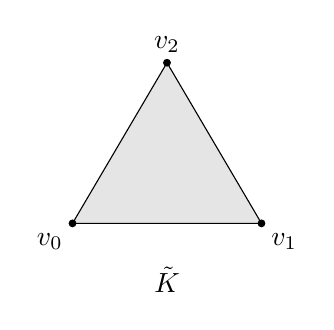
\begin{tikzpicture}[scale=1.2]
\fill[gray!20] (0,0) -- (2,0) -- (1,1.7) -- cycle;
\filldraw[black] (0,0) circle (1pt) node[below left] {\(v_0\)};
\filldraw[black] (2,0) circle (1pt) node[below right] {\(v_1\)};
\filldraw[black] (1,1.7) circle (1pt) node[above] {\(v_2\)};
\draw (0,0) -- (2,0) -- (1,1.7) -- cycle;
\node at (1,-0.6) {\textbf{\(\tilde{K}\)}};
\end{tikzpicture}
\end{center}
Se puede probar que las realizaciones geométricas de complejos simpliciales finitos son homeomorfas a subespacios de $\mathbb{R}^n$ (en el sentido topológico, es decir, un subconjunto de $\mathbb{R}^n$ dotado de la topología subespacio) para algún $n$.
\\
\subsubsection{Complejo de cadenas simplicial}
Si $K$ es un complejo simplicial, para cada $n$ tomamos $C_n(K)$ como el grupo abeliano libre generado por los $n$-símplices orientados $[v_0, \ldots, v_n]$ de $K$.
\\
\\
Definimos el \textit{borde} de un $n$-símplex orientado como
\[
\partial_n([v_0, \ldots, v_n]) = \sum_{i=0}^{n}(-1)^i \, [v_0, \ldots, \hat{v_i}, \ldots, v_n]
\]
donde $[v_0, \ldots, \hat{v_i}, \ldots, v_n]$ es el $(n-1)$-símplex que se obtiene borrando el vértice $i$-ésimo.
\\
\\
Se obtiene así el complejo de cadenas $(C_*(K), \partial_*)$
\[
\ldots \rightarrow C_n(K) \xrightarrow{\partial_n} C_{n-1}(K) \rightarrow \ldots \rightarrow C_2(K) \xrightarrow{\partial_2} C_1(K) \xrightarrow{\partial_1} C_0(K) \rightarrow 0
\]
al que llamamos \textit{complejo simplicial de $K$} y a partir del cual calculamos $H_*(K)$, la \textit{homología simplicial de $K$}.
\\
\\
\\
Veamos un ejemplo de cómo se calcula, en la práctica, el morfismo de borde.
\\
\\
Sea $K$ el complejo simplicial definido previamente: sus 0-símplices son $\{[v_0], [v_1], [v_2]\}$ y sus 1-símplices $\{[v_0, v_1], [v_1,v_2], [v_0,v_2]\}$. No tiene 2-símplices (ni $n$-símplices para ningún $n>2$).
\begin{center}
\begin{minipage}{0.3\linewidth}
\centering
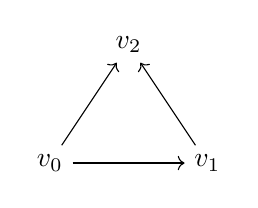
\begin{tikzpicture}[->, scale=1]
  % Vértices
  \node (v0) at (0,0) {$v_0$};
  \node (v1) at (2,0) {$v_1$};
  \node (v2) at (1,1.5) {$v_2$};

  % Flechas
  \draw (v0) -- (v1);
  \draw (v0) -- (v2);
  \draw (v1) -- (v2);
\end{tikzpicture}
\end{minipage}%
\begin{minipage}{0.5\linewidth}
\centering
$C_0(K) = <v_0, v_1, v_2>$
\\
$C_1(K) = <[v_0 v_1], [v_1v_2], [v_0v_2]>$
\\
$C_2(K) = 0$
\end{minipage}
\end{center}
Su complejo de cadenas resulta
\[
    \ldots \rightarrow 0 \xrightarrow{\partial_n} 0 \rightarrow \ldots \rightarrow 0 \xrightarrow{\partial_2} <[v_0 v_1], [v_1v_2], [v_0v_2]> \xrightarrow{\partial_1} <v_0, v_1, v_2> \rightarrow 0
\]
\\
Supongamos que queremos calcular la homología 1-ésima de $K$. Para eso, necesitamos calcular el núcleo de $\partial_1$ y la imagen de $\partial_2$.
\\
\\
Por un lado, como $\partial_2$ es un morfismo, $\text{Im}(\partial_2) = 0$. Por el otro, sea $\sigma = [v_iv_j] \in C_1(K)$ uno de sus generadores.
\\
\\
Es claro que $\sigma^{(0)} = v_j$, $\sigma^{(1)} = v_i$, luego $\partial_1$ es tal que
\[
\partial_1(\sigma) = (-1)^0.\sigma^{(0)} + (-1)^1.\sigma^{(1)} = \sigma^{(0)} - \sigma^{(1)} = v_j - v_i
\]
Para calcular su núcleo, tomemos un $\alpha = a[v_0v_1] + b[v_1v_2] + c[v_0v_2] \in C_1(K)$, con $a, b, c \in \mathbb{Z}$ y veamos qué condiciones necesitamos para que $\partial_1(\alpha) = 0$.
\\
\\
Por cómo definimos los morfismos de borde, $\partial_1(\alpha) = a.(v_1-v_0) + b.(v_2-v_1) + c.(v_2-v_0)$. Resolviendo el sistema, resulta $\partial_1(\alpha)=0$ si y sólo si $b = a$ y $c = -a$. Es decir, si y sólo si $\alpha = a.([v_0v_1] + [v_1v_2] - [v_0v_2])$, con $a \in \mathbb{Z}$.
\\
\\
Así, $\ker(\partial_1)=\mathbb{Z}<[v_0v_1] + [v_1v_2] - [v_0v_2]> \simeq \mathbb{Z}$.
\\
\\
Podemos concluir entonces que $H_1(K) = \mathbb{Z} / 0 = \mathbb{Z}$, lo que coincide con nuestra intuición de que el triángulo sin relleno tiene un agujero de dimensión 1.
\\
\\
\subsection{Homología singular}
Algunas definiciones previas sobre $A$-módulos:
\begin{definition}    
Un \textit{anillo} $A$ es una terna $(A, +, \cdot)$, con $A$ un conjunto tal que $(A, +)$ es un grupo abeliano y $(A, \cdot)$ es un semigrupo.
\end{definition}
Notar que un anillo, a diferencia de un cuerpo, no necesariamente tiene un inverso multiplicativo para todos sus elementos no nulos.
\begin{definition}    
Un \textit{$A$-módulo} generaliza el concepto de espacio vectorial sobre un cuerpo, pero definido sobre un anillo $A$.
\end{definition}
\medskip
\subsubsection{Complejo de cadenas singular}
\begin{definition}    
Sea $X$ un espacio topológico. Sea $n \geq 0$. Un $n$-\textit{símplex singular} en $X$ es una función continua $\sigma: \triangle^n \rightarrow X$.
\end{definition}
Por un lado, definimos $C_n(X)$ como el $\mathbb{Z}$-módulo libre generado por los $n$-símplices singulares de $X$. Es decir,
\[
C_n(X) = \{\sum_{finita} n_\sigma\sigma : n_\sigma \in \mathbb{Z} \text{ con } \sigma: \triangle^n \rightarrow X \text{ continua}\}
\]
Por el otro, definimos el morfismo de borde $\partial_n : C_n(X) \rightarrow C_{n-1}(X)$ en la base como
\[
\partial_n(\sigma) = \sum_{i=0}
^n(-1)^i \sigma|_{[v_0 \ldots \hat{v_i} \ldots v_n]}
\]
Se tiene así un complejo de cadenas $(C_*(X), d)$
\[
\ldots \rightarrow C_n(X) \xrightarrow{\partial_n} C_{n-1}(X) \rightarrow \ldots \rightarrow C_2(X) \xrightarrow{\partial_2} C_1(X) \xrightarrow{\partial_1} C_0(X) \rightarrow 0
\]
al que llamamos \textit{complejo singular de $X$} y a partir del cual calculamos $H_n(X)$, la \textit{homología singular de $X$}.
\\
\\
\subsubsection{Homología singular relativa}
Sea $A \subseteq X$ un subespacio (topológico). Consideramos el subcomplejo $C_*(A) \subseteq C_*(X)$, donde a los símplices singulares de $A$ los podemos pensar como los símplices singulares de $X$ cuyas imágenes caen en $A$.
\\
\\
Así, tenemos una S.E.C. de complejos
\[
0 \rightarrow C_*(A) \xrightarrow{i} C_*(X) \xrightarrow{q} C_*(X)/C_*(A) \rightarrow 0
\]
donde el ``complejo cociente'' $C_*(X)/C_*(A)$ se define como la sucesión de módulos cocientes $C_n(X)/C_n(A)$, y los morfismos de borde $\overline{\partial_n}$ como los inducidos por $\partial_n$ en el cociente.
\\
\\
Es decir, supongamos $\overline{x} \in C_n(X)/C_n(A)$. Como $x \in C_n(X)$, sabemos calcular $\partial_n(x) \in C_{n-1}(X)$. Más aún, sabemos tomarle clase en el cociente $C_{n-1}(X)/C_{n-1}(A)$. Por lo tanto podemos definir $\overline{\partial_n}(\overline{x}) \coloneqq \overline{\partial_n(x)} \in C_{n-1}(X)/C_{n-1}(A)$.
\begin{definition}
Dado $A \subseteq X$, se define la \textit{homología singular relativa} del par $(X,A)$ como $H_n(X,A) \coloneqq H_n(C_*(X)/C_*(A))$.
\end{definition}
La sucesión exacta corta definida previamente induce entonces una sucesión exacta larga en las homologías:
\[
\ldots \rightarrow H_n(A) \xrightarrow{i_n} H_n(X) \xrightarrow{q_n} H_n(X,A) \xrightarrow{\partial_n} H_{n-1}(A) \xrightarrow{i_{n-1}} H_{n-1}(X) \xrightarrow{q_{n-1}} H_{n-1}(X,A) \ldots
\]
\[
\ldots \rightarrow H_0(A) \xrightarrow{i_0} H_0(X) \xrightarrow{q_0} H_0(X,A) \rightarrow 0
\]
\subsubsection{Morfismos inducidos}
\begin{proposition}
Sea $f: X \rightarrow Y$ una función continua. Entonces $f$ induce un morfismo de complejos $f_*: C_*(X) \rightarrow C_*(Y)$, y por lo tanto $f_*$ es un morfismo de complejos de cadenas que induce morfismos entre las homologías $f_n: H_n(X) \rightarrow H_n(Y) \quad \forall n \geq 0$.
\end{proposition}
\begin{proof}
Para cada $n \geq 0$, dada $\sigma : \triangle^n \rightarrow X$ continua, definimos 
\[
f_*(\sigma) \coloneqq f\sigma : \triangle^n \xrightarrow{\sigma} X \xrightarrow{f} Y
\]
y extendemos linealmente $f_*(\sum n_\sigma \sigma) = \sum n_\sigma f \sigma$.
\\
Notar que $f_*$ conmuta con el morfismo de borde pues
\[
f_*(d_n(\sigma)) = f_*(\sum_{i=0}^n(-1)^i \sigma^{(i)}) = \sum_{i=0}^n(-1)^i f_*(\sigma^{(i)}) = \sum_{i=0}^n(-1)^i (f\sigma)^{(i)} = d_n(f_*(\sigma))
\]
Además, la asignación es functorial pues $(fg)_* = f_*g_*$, $(1_X)_* = 1_{C_*(X)}$. Y por lo tanto si $f$ es un homeomorfismo, $f_*$ es un isomorfismo de complejos y $f_n$ un isomorfismo entre las homologías.
\end{proof}
Vale lo mismo para homología reducida.
\begin{definition}
Sean $f_*, \, g_* : C_* \rightarrow C'_*$ morfismos de complejos. Una \textit{homotopía} $h_*: f_* \simeq g_*$ es una familia de morfismos $h_n: C_n \rightarrow C'_{n+1} \, \forall n$, tales que $f_n - g_n = d'_{n+1}h_n + h_{n-1}d_n$.
\[
\begin{tikzcd}[column sep=large, row sep=large]
\cdots \arrow[r] 
  & C_{n+1} 
    \arrow[r, "d_{n+1}"] 
    \arrow[d, shift right=0.5ex, "f"'] 
    \arrow[d, shift left=0.5ex, "g"] 
  & C_n 
    \arrow[r, "d_n"] 
    \arrow[d, shift right=0.5ex, "f"'] 
    \arrow[d, shift left=0.5ex, "g"] 
    \arrow[dl, "h_n"] 
  & C_{n-1} 
    \arrow[r] 
    \arrow[d, shift right=0.5ex, "f"'] 
    \arrow[d, shift left=0.5ex, "g"] 
    \arrow[dl, "h_{n-1}"] 
  & \cdots \\
\cdots \arrow[r] 
  & C'_{n+1} \arrow[r, "d'_{n+1}"] 
  & C'_n \arrow[r, "d'_n"] 
  & C'_{n-1} \arrow[r] 
  & \cdots
\end{tikzcd}
\]
\end{definition}
Observemos que $\simeq$ es una relación de equivalencia en el conjunto de morfismos de $C_*$ a $C'_*$ pues:
\\
\\
1. Si $h_n \equiv 0$, entonces $f_n - f_n = 0$ y por lo tanto $f_* \simeq f_*$.
\\
\\
2. Si $h_*: f_* \simeq g_*$ entonces $g_n - f_n = -(f_n - g_n) = -(d'_{n+1}h_n + h_{n-1}d_n) = d'_{n+1}(-h_n) + (-h_{n-1})d_n$ y por lo tanto $-h_*: g_* \simeq f_*$.
\\
\\
3. Si $h_*: f_* \simeq g_*$, entonces $l_*: g_* \simeq r_*, \, f_n - r_n = (f_n - g_n) + (g_n-r_n) = (d'_{n+1}h_n + h_{n-1}d_n) + (d'_{n+1}l_n + l_{n-1}d_n) = \ldots = d'_{n+1}(h_n + l_n) + (h_{n-1} + l_{n-1})d_n$, y por lo tanto $h_* + l_*: f_* \simeq r_*$.
\begin{proposition}
Sean $f_*,g_*: C_* \rightarrow C'_*$ morfismos de complejos. Si $f_* \simeq g_*$, vale que $f_n = g_n : H_n(C) \rightarrow H_n(C') \, \forall n$
\end{proposition}
\begin{theorem}
Sean $f,g : X \rightarrow Y$ continuas. Si $f \simeq g$ entonces $f_* \simeq g_* :C_*(X) \rightarrow C_*(Y)$, y en ese caso $f_n = g_n: H_n(X) \rightarrow H_n(Y)$ para todo $n \geq 0$.
\\
Es decir, funciones homotópicas inducen morfismos homotópicos a nivel complejos. 
\end{theorem}
\begin{proof}
Sea $h:X \times I \rightarrow Y, h: f \simeq g$. Debemos ver que existe $h_* : f_* \simeq g_*$, es decir, que existen $h_n: C_n(X) \rightarrow C_{n+1}(Y)$ para todo $n$ tales que $f_n - g_n = d^Y_{n+1}h_n + h_{n-1}d^X_n$.
\\
\\
Dada $\sigma: \triangle^n \rightarrow X$ continua, consideramos $h(\sigma \times 1_I): \triangle^n \times I \rightarrow Y$.
\\
El ``prisma'' $\triangle^n \times I$ tiene como vértices a los de $\triangle^n \times \{0\}$ que denotamos $[v_0,\ldots,v_n]$ y a los de $\triangle^n \times \{1\}$ que denotamos $[w_0,\ldots,w_n]$.
\\
Podemos subdividirlo en $n+1 \, (n+1)$-símplices. Es decir,
\[
\triangle^n \times I : \bigcup_{i=0}^n [v_0 \ldots v_i w_i \ldots w_n]
\]
Si definimos $\displaystyle h_*(\sigma) = \sum_{i=0}^n(-1)^i h(\sigma \times I)|_{[v_0 \ldots v_i w_i \ldots w_n]}$, se tiene que $(dh_*+h_*d)(\sigma) = g\sigma - f\sigma$, y por lo tanto $h_*: g_* \simeq f_*, \, -h_* : f_* \simeq g_*$.
\end{proof}
\begin{corollary}
Si $f: X \rightarrow Y$ es una equivalencia homotópica, $f_n : H_n(X) \rightarrow H_n(Y)$ es un isomorfismo para todo $n$.
\end{corollary}
\newpage
\subsection{Homología celular}
Queremos construir espacios ``pegando'' puntos de distintos espacios.
\begin{definition}
    Sean $X$, $Y$ espacios topológicos. Sea $A \subseteq X$ subespacio (topológico) cerrado y $f: A \rightarrow Y$ una función continua. El espacio de adjunción $Y \, \cup_f \, X$ se define a partir de la unión disjunta $Y \bigsqcup X$, identificando los puntos $a \in A$ con los puntos $f(a) \in Y$. A $f$ la llamamos función de adjunción.
    \\
    \\
    Formalmente, $Y \cup_f X \coloneqq Y \bigsqcup X /\sim$, con $a \sim f(a) \quad \forall a \in A$.
\end{definition}
Sean $q$ la función cociente $q: Y \bigsqcup X \rightarrow Y \cup_f X$, $i_Y$ la inclusión de $Y$ en $Y \bigsqcup X$, $i_X$ la inclusión de $X$ en $Y \bigsqcup X$. Si $\overline{i} = q \circ i_Y$, $\overline{\alpha} = q \circ i_X$, se tiene el siguiente diagrama conmutativo:
\[
\begin{tikzcd}
A \arrow[r, "f"] \arrow[d, "i"] & Y \arrow[d, "\overline{i}"] \\
X \arrow[r, "\overline{\alpha}"]           & Y \, \cup_f \, X
\end{tikzcd}
\]
Notar que, como $Y \bigsqcup X$ tiene la topología final respecto de las inclusiones de $Y$ y $X$ y $q$ es en particular final, entonces $Y \cup_f X$ tiene la topología final respecto de las funciones $\overline{i}$ y $\overline{\alpha}$. Es decir, $U \subseteq Y \cup_f X$ es abierto si y sólo si $\overline{i}^{-1}(U) \subseteq Y$ y $\overline{\alpha}^{-1}(U) \subseteq X$ son abiertos.
\begin{definition}
Un espacio es una \textit{celda} de dimensión $n$, o una $n$-celda, si es homeomorfo a $B^n$. A una $n$-celda la notamos $e^n$.
\end{definition}
Sean $X = \mathbb{D}^n$ el disco relleno de dimensión $n$, $A = \partial \mathbb{D}^n = \mathbb{S}^{n-1}$. Sea $f: \partial \mathbb{D}^n \rightarrow Y$ una función continua. Decimos que el espacio de adjunción $Y \cup_f \mathbb{D}^n$ se obtiene de $Y$ \textit{adjuntándole una $n$-celda}, y lo notamos $Y \cup e^n$:
\[
\begin{tikzcd}
\mathbb{S}^{n-1} \arrow[r, "f"] \arrow[d, "i"] & Y \arrow[d, "\overline{i}"] \\
\mathbb{D}^n \arrow[r, "\overline{\alpha}"]           & Y \cup e^n
\end{tikzcd}
\]
La función $\overline{\alpha}$ se llama \textit{función característica de la celda}, y la $n$-celda $e^n$ es la imagen de $\mathbb{D}^n$ vía $\overline{\alpha}$, es decir, $e^n = \overline{\alpha}(\mathbb{D}^n)$.
\\

Notar que $\overline{\alpha}|_{(\mathbb{D}^n)^\circ} : (\mathbb{D}^n) ^\circ \rightarrow (e^n)^\circ$ es un homeomorfismo. Es decir, los interiores de las celdas son homeomorfos a discos abiertos. 
\subsubsection{Complejos CW}
\begin{definition}
Sea $X$ un espacio topológico. Decimos que el par $(X, \mathcal{E})$ es una \textit{descomposición celular de $X$} si $\mathcal{E}$ es una partición de $X$ en celdas. Es decir, si cada elemento de $\mathcal{E}$ es una celda, $X$ es la unión de todos los elementos de $\mathcal{E}$ y todos los elementos en $\mathcal{E}$ son disjuntos.
\end{definition}
\begin{definition}
Sea $(X, \mathcal{E})$ una descomposición celular. Decimos que es, además, un \textit{CW-complejo} si se cumplen las siguientes condiciones:
\begin{enumerate}
    \item $X$ es Hausdorff.
    \item Para cada $e^n \in \mathcal{E}$, su función característica es tal que $\overline{\alpha}_e(\mathbb{S}^{n-1})$ es una unión finita de células, cada una de dimensión menor a $n$.
    \item $X$ tiene la topología débil con respecto a $\mathcal{E}$: 
    un subconjunto $U \subseteq X$ es abierto si y sólo si para todo $e$ 
    se cumple que $U \cap e$ es abierto en $e$.
\end{enumerate}
\end{definition}
Las dos últimas condiciones son el origen de las letras $C$ y $W$ de los \textit{\textbf{C}losure finite \textbf{W}eak topology} complejos.
\\
\\
Veamos ahora cómo computar la homología singular de un CW-complejo. Para simplificar notación, $X$ denotará un CW-complejo con un conjunto $\mathcal{E}$ de celdas y funciones características $\overline{\alpha}_e$.
\subsubsection{Complejo de cadenas celular}
\begin{definition}
Dado $n > 0$, definimos $X^n$ como el espacio que se obtiene de $X^{n-1}$ adjuntándole las $n$-celdas de $\mathcal{E}$. Lo llamamos el \textit{$n$-esqueleto} de $X$. Los elementos de $X^0$ se llaman $0$-celdas y forman un espacio discreto.
\end{definition}
Es claro que $X^{n-1} \subseteq X^n$. Además, si existe $n$ tal que $X^n = X$, decimos que $X$ tiene dimensión finita. En caso contrario, tiene dimensión infinita.
\begin{definition}
Si $X$ es un CW-complejo, definimos la homología relativa del par $(X^n, X^{n-1})$ como $D_n(X) = H_n(X^n, X^{n-1})$, donde para cada $n$ el morfismo de borde $\partial_n: D_n(X) \rightarrow D_{n-1}(X)$ se define como la composición $i_n \circ \partial_n^{rel}$:
\[
H_n(X^n, X^{n-1}) \xrightarrow{\partial_n^{rel}} H_{n-1}(X^{n-1}) \xrightarrow{i_n} H_{n-1}(X^{n-1}, X^{n-2})
\]
\end{definition}
Notar que $\partial_n^2 = 0$.
\begin{definition}
Definimos el \textit{complejo celular de cadenas de $X$} al complejo de cadenas $(D_\bullet(X), \partial_\bullet)$.
\end{definition}
Este complejo se puede usar para computar la homología singular de $X$ utilizando los siguientes lemas:
\begin{lemma}
    Si $X$ es un CW-complejo, entonces
    \[
    H_k(X^n, X^{n-1}) =
    \begin{cases}
    0 & k \neq n\\[2mm]
    \mathbb{Z}^{\#\text{n-celdas}} & k = n
    \end{cases}
    \qquad \text{y } \quad
    H_k(X^n) = 0 \quad k > n
    \]
\end{lemma}
\begin{lemma}
    Si $X$ es un CW-complejo, entonces
    \[
    H_k(D_\bullet(X), \partial_\bullet) = H_k(X)
    \]
\end{lemma}
Veamos cómo, utilizando estos lemas, podemos calcular la homología celular de $\mathbb{S}^1$: consideremos la descomposición celular que consta de una $0$-celda $e^0$ y una $1$-celda $e^1$, con sus respectivas funciones características. Notar que $X^1$ es el espacio que se obtiene adjuntándole $e^1$ a $e^0$, y que $X^0 = e^0$.
\begin{center}
% S^1 completo a la izquierda
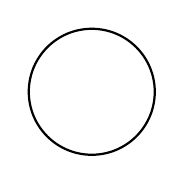
\begin{tikzpicture}[scale=0.8]
  \draw[thick] (0,0) circle (1); 
\end{tikzpicture}
\hspace{2cm} % espacio entre los dibujos
% Descomposición celular a la derecha
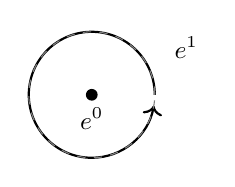
\begin{tikzpicture}[scale=1]
  % 0-celda
  \node[fill=black,circle,inner sep=1.5pt] (v) at (0,0) {};
  \node at (0,-0.3) {\small $e^0$};
  
  % 1-celda: bucle alrededor del vértice
  \draw[thick,->] (0.8,0) arc (0:350:0.8); 
  \node at (1.2,0.6) {\small $e^1$};
  
  % referencia del círculo completo como guía
  \draw[dashed, gray] (0,0) circle (0.8);
\end{tikzpicture}
\end{center}
Como $X^1$ sólo tiene una $1$-celda y $X_0$ sólo tiene una $0$-celda, resulta
\[
H_1(X^1, X^0) \cong \mathbb{Z}, \qquad H_0(X^0, X^{-1}) \cong \mathbb{Z}
\]
Y por lo tanto
\[
H_1(\mathbb{S}^1) \cong H_1(X^1, X^0) \cong \mathbb{Z}, \qquad H_0(\mathbb{S}^1) \cong H_0(X^0, X^{-1}) \cong \mathbb{Z}
\]
En el siguiente capítulo introduciremos los conceptos de filtración y módulos de persistencia, dos nociones fundamentales para el estudio de la homología persistente.
\\
\\
\subsection{Filtraciones y módulos de persistencia}
Definiremos, primero, nociones generales para espacios topológicos y espacios vectoriales.
\begin{definition}
    Sea $I \subseteq \mathbb{R}$. Una \textit{filtración} de espacios topológicos es una colección $X = (X_r)_{r \in I}$ de espacios topológicos e inclusiones $X_{r,s}: X_r \rightarrow X_s$ para $r \leq s$.
\end{definition}
\begin{definition}
    Sea $I \subseteq \mathbb{R}$. Una \textit{filtración} de espacios vectoriales es una colección $V = (V_r)_{r \in I}$ de espacios vectoriales e inclusiones $V_{r,s}: V_r \rightarrow V_s$ para $r \leq s$. En este caso, una base $B$ de $V$ es una colección de subconjuntos $B_r \subseteq V_r$ tales que $B_r$ es una base de $V_r$ y $B_r \subseteq B_s$ si $r \leq s$.
\end{definition}
\begin{definition}
    Un morfismo $\phi: X \rightarrow Y$ entre filtraciones -de espacios topológicos o vectoriales- indexadas en $I$ es una colección de funciones $\phi_r: X_r \rightarrow Y_r$ tales que $\phi_r$ conmuta con las inclusiones, es decir, $\phi_s \circ X_{r,s} = Y_{r,s} \circ \phi_r $ para todo $r \leq s$.
\end{definition}
\begin{definition}
    Un \textit{módulo de persistencia} indexado en $I \subseteq \mathbb{R}$ es una colección $(V_r)_{r \in I}$ de espacios vectoriales junto con morfismos $V_{r,s}: V_r \rightarrow V_s$ para $r \leq s$ tales que $V_{r,t} = V_{s,t} \circ V_{r,s}$ si  $r \leq s \leq t$, a los que llamamos de estructura.
\end{definition}
\begin{definition}
    Sean $V$ y $W$ módulos de persistencia indexados en $I \subseteq \mathbb{R}$. Un morfismo de módulos de persistencia $\phi:V \rightarrow W$ es una colección de funciones lineales $\phi_r : V_r \rightarrow W_r$ que conmutan con las funciones de estructura. Es decir, $\phi_s \circ V_{r,s} = W_{r,s} \circ \phi_r $ para todo $r \leq s$, con $r, s \in I$.
\end{definition}
\begin{definition}
    Sea $V$ un módulo de persistencia indexado en $I$. Para cada $i \in I$, definimos $V^\dagger_i \coloneqq \{v \in V_i :  V_{i,q}(v) = 0\}$ (elementos que desaparecen en algún momento) y $V^\infty_i \coloneqq V_i / V_i^\dagger$ (elementos que persisten).
\end{definition}
Notar que $\overline{v} = \overline{u}$ en $V^\infty_i$ si ${v-u} \in V_i^\dagger$.
\begin{proposition}
    $(V^\dagger_i)_{i \in I}$ y $(V^\infty_i)_{i \in I}$ son módulos de persistencia.
\end{proposition}
\begin{proof}
    Veamos, en primer lugar, que $(V^\dagger_i)_{i \in I}$ lo es. Es decir, queremos ver que es una colección de espacios vectoriales junto con morfismos de estructura $V_{r,s}^\dagger: V_r^\dagger \rightarrow V_s^\dagger$ para $r \leq s$ tales que $V_{r,t}^\dagger = V_{s,t}^\dagger \circ V_{r,s}^\dagger$ si $r \leq s \leq t$.
    \\
    \\
    Notemos que un elemento que desaparece no vuelve a aparecer. Es decir que, si $v$ es tal que $V_{i,q}(v) = 0$, entonces para todo $\tilde{q} \geq q$ vale que $V_{i, \tilde{q}}(v) = 0$. En efecto, como $V$ es un módulo de persistencia, en particular vale que $V_{i,\tilde{q}} = V_{q, \tilde{q}} \circ V_{i,q}$. Como $V_{q,\tilde{q}}(0) = 0$ por linealidad de los morfismos, resulta $V_{i,\tilde{q}}(v) = 0$. Utilizando estos mismos argumentos es fácil ver que $V_i^\dagger$ es un espacio vectorial para cada $i$.
    \\
    \\
    Luego $V_i^\dagger$ es un subconjunto de $V_i$ y además es un espacio vectorial, y por lo tanto es un subespacio de $V_i$. Así que podemos definir a nuestros morfismos de estructura como la restricción al subespacio, es decir, $V_{r,s}^\dagger \coloneqq V_{r,s}|_{V_r^\dagger}$.
    \\
    \\
    \\
    En segundo lugar, veamos que $(V_i^\infty)_{i \in I}$ es un módulo de persistencia. En efecto, como el cociente entre espacios vectoriales es un espacio vectorial, para cada $i \in I$ fijo $V_i^\infty \coloneqq V_i / V_i^{\dagger}$ resulta un espacio vectorial.
    \\
    \\
    Dados $r \leq s$ y $\overline{v} \in V_r^{\infty}$, definimos $V_{r,s}^{\infty}(\overline{v}) \coloneqq \overline{V_{r,s}(v)} \in V_s^{\infty}$, que está bien definido por las propiedades de $V_{r,s}$ y $V_{r,s}^{\dagger}$. Es claro, además, que $V_{r,t}^{\infty} = V_{s,t}^{\infty} \circ V_{r,s}^{\infty}$.
\end{proof}
Definimos a $V^\infty \coloneqq (V^\infty_i)_{i \in I}$ como la \textit{parte inmortal de $V$} y a $V^\dagger \coloneqq (V^\dagger_i)_{i \in I}$ como la \textit{parte mortal de $V$}.
\begin{proposition}
    Sea $\phi:V \rightarrow W$ un morfismo de módulos de persistencia.
    \\
    Si $W$ es una filtración de espacios vectoriales, vale que $im\phi$ es una filtración de espacios vectoriales y que, para calcularla, podemos restringirnos a su parte inmortal. Es decir, $im\phi = im\phi|_{V^\infty}$
\end{proposition}
\begin{proof}
    En primer lugar, veamos que $\text{im}\phi$ es una filtración de espacios vectoriales. Es decir, que es una colección $(\text{im} (\phi_r))_r$ de espacios vectoriales tales que $\text{im}\phi_r \subseteq \text{im}\phi_s$ si $r \leq s$, e inclusiones $\text{im}\phi_{r,s}: \text{im}\phi_r \rightarrow \text{im}\phi_s$.
    \\
    \\
    Sea $r \in I$ fijo. Como $\phi_r: V_r \rightarrow W_r$ y $V_r$ y $W_r$ son espacios vectoriales, $\text{im}\phi_r$ es un espacio vectorial. Dados $r \leq s \in I$, por conmutatividad vale que $\phi_s \circ V_{r,s} = W_{r,s} \circ \phi_r$. Como $W_{r,s}$ es una inclusión, $\text{im}\phi_r = \text{im}(W_{r,s} \circ \phi_r)$. Por lo tanto $\text{im}\phi_r = \text{im} (\phi_s \circ V_{r,s}) \subseteq \text{im}\phi_s$.
    \\
    \\
    En segundo lugar, veamos que $\text{im} \phi = \text{im}\phi|_{V^\infty}$. Notemos que un módulo de persistencia es la suma directa entre su parte mortal e inmortal. En efecto, como para cada $i \in I$ es $V_i = V^\infty_i \oplus V^\dagger_i$, tenemos que $V = (V_i)_{i \in I} = (V^\infty_i \oplus V^\dagger_i)_{i \in I} = (V^\infty_i)_{i \in I} \oplus (V^\dagger_i)_{i \in I} = V^\infty \oplus V^\dagger$, y por lo tanto basta entonces ver que $\text{im} (\phi|_{V^\dagger}) = 0$,  es decir, que para cada $i$ es $\text{im} (\phi_i|_{V_i^\dagger}) = 0$.
    \\
    \\
    Dados $i \in I$ y $v \in V_i^\dagger$, queremos ver que $\phi_i(v) = 0$. Como $v \in V_i^\dagger$ existe $q$ tal que $V_{i,q}(v) = 0$. Por el mismo razonamiento utilizado anteriormente, $\phi_i(v) = (W_{i,q} \circ \phi_i)(v) = (\phi_q \circ V_{i,q})(v)$. Y como $V_{i,q}(v) = 0$ y $\phi_q$ es lineal resulta $\phi_i(v) = 0$, que era lo que queríamos.
\end{proof}
\begin{definition}
    Un módulo de persistencia indexado en $\mathbb{Z}$ es una colección de espacios vectoriales $(V_i)_{i \in \mathbb{Z}}$ junto con morfismos $\{ \phi_i : V_i \rightarrow V_{i+1} \}$ tales que $V_{i,l} = V_{j,l} \, \circ \, V_{i,j}$ si $i \leq j \leq l$.
    Dados $i \leq j$, notamos $\phi^{i \rightarrow j}: V_i \rightarrow V_j$ a la composición $\phi_{j-1} \circ \phi_{j-2} \circ \dots \circ \phi_{i+1} \circ \phi_{i}$.
\end{definition}
Notar que un módulo de persistencia así no es necesariamente un complejo de cadenas, ya que no siempre se cumple la condición $\phi_i \circ \phi_{i-1} = 0$.
\begin{definition}
    Decimos que $v \in V_i$ \textit{nace} en el parámetro $i$ si $v \notin \text{im}\phi_{i-1}$.
    \\
    Decimos que $v \in V_i$ \textit{muere} en el parámetro $j \geq i$ si $j = \min \{k : \phi^{i \rightarrow k}(v) = 0\}$. Si no existe tal $j$, notamos $+\infty$ al parámetro de muerte.
\end{definition}
Ahora sí, estamos en condiciones de dar la definición de filtración para complejos simpliciales, que es la que necesitaremos para el cálculo de homología persistente:
\begin{definition}
    Sea $K$ un complejo simplicial. Una filtración de complejos simpliciales para $K$ es una colección de complejos simpliciales $\{K_n\}_{n=0}^N$ tales que $K_i \subseteq K_{i+1}$ y $K_N = K$.
\end{definition}
La functorialidad de la homología induce un módulo de persistencia asociado a nuestra filtración. En efecto, si $\{K_n\}_n$ es una filtración de un complejo simplicial $K$, y $i_n: K_n \rightarrow K_{n+1}$ son los morfismos inclusión, los morfismos inducidos
\[
(i_n)_* : H_k(K_n, \mathbb{F}) \rightarrow H_k(K_{n+1}, \mathbb{F})
\]
nos permiten construir el módulo de persistencia
\[
H_k(K_0, \mathbb{F}) \xrightarrow{(i_0)_*} H_k(K_1, \mathbb{F}) \xrightarrow{(i_1)_*} \ldots \xrightarrow{(i_{N-2})_*} H_k(K_{N-1}, \mathbb{F}) \xrightarrow{(i_{N-1})_*} H_k(K_N, \mathbb{F}) = H_k(K, \mathbb{F})
\]
Más aún, para $i < j$ tenemos la inclusión
\[
i^{i\rightarrow j} \coloneqq i_j \circ i_{j-1} \circ \ldots \circ i_{i+1} \circ i_i : K_i \rightarrow K_j
\]
que induce un morfismo en la homología
\[
(i^{i \rightarrow j})_* : H_k(K_i, \mathbb{F}) \rightarrow H_k(K_j, \mathbb{F})
\]
\section{Homología persistente}
Supongamos que queremos calcular la homología de un espacio topológico $X$, pero lo único que tenemos es $(X_n,d)$ una muestra finita de $X$. Quisiéramos inferir la homología de $X$ a partir de la de $X_n$.
\begin{definition}    
    Un estimador de $X$ a partir de $X_n$ es $\displaystyle U_\varepsilon \coloneqq \bigcup_{x \in X_n} B_\varepsilon(x)$ para algún $\varepsilon > 0$.
\end{definition}
\begin{figure}[h!]
\centering
\begin{subfigure}{0.3\textwidth}
\centering

\begin{tikzpicture}[scale=0.4]
  \def\R{2.5}
  \draw[thick, gray!70] (0,0) circle[radius=\R];
\end{tikzpicture}
\caption*{$X$}
\end{subfigure}
\hfill
\begin{subfigure}{0.3\textwidth}
\centering
\begin{tikzpicture}[scale=0.4]
  \def\R{2.5}
  \draw[dashed, gray!50] (0,0) circle[radius=\R];
  \foreach \ang/\name in {
    15/A, 50/B, 78/C, 110/D, 155/E, 195/F, 228/G, 255/H, 305/I, 345/J}
  {
    \coordinate (\name) at ({\R*cos(\ang)},{\R*sin(\ang)});
    \fill[black] (\name) circle[radius=0.6mm];
  }
\end{tikzpicture}
\caption*{$X_n \subseteq X$}
\end{subfigure}
\hfill
\begin{subfigure}{0.3\textwidth}
\centering
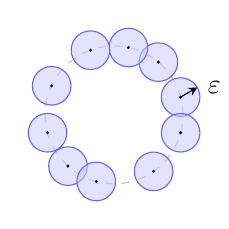
\begin{tikzpicture}[scale=0.35]
  \def\R{2.5}
  \def\eps{0.7}
  \draw[dashed, gray!50] (0,0) circle[radius=\R];
  \foreach \ang/\name in {
    15/A, 50/B, 78/C, 110/D, 155/E, 195/F, 228/G, 255/H, 305/I, 345/J}
  {
    \coordinate (\name) at ({\R*cos(\ang)},{\R*sin(\ang)});
    \fill[blue!20,opacity=0.55] (\name) circle[radius=\eps];
    \draw[blue!60, thin] (\name) circle[radius=\eps];
    \fill[black] (\name) circle[radius=0.6mm];
  }
  \draw[->, >=stealth] (A) -- ++({\eps*cos(30)}, {\eps*sin(30)});
    \node[right,overlay] at ($(A)+(\eps*0.9, \eps*0.5)$) {$\varepsilon$};
\end{tikzpicture}
\caption*{$U_{\varepsilon}$}
\end{subfigure}
\end{figure}
Supongamos que tenemos un estimador. ¿Cómo ``recuperamos'' el espacio subyacente? Es decir, ¿bajo qué hipótesis de $\varepsilon$ nos aseguramos de que la homología de $U_\varepsilon$ coincide con la de $X$? Y más aún: aún teniendo estas hipótesis, ¿cómo encontramos el $\varepsilon$ que nos sirve?
\\

Evidentemente, en la práctica encontrar el $\varepsilon$ buscado es difícil. La idea de la \textit{homología persistente} es estudiar los generadores de la homología de $U_\varepsilon$ que \textit{persisten} en los distintos valores de $\varepsilon$. Es decir, características topológicas persistentes en $\{U_\varepsilon : \varepsilon > 0\}$: notar que, si $\varepsilon' < \varepsilon$, $U_{\varepsilon'} \subseteq U_\varepsilon$, y por functorialidad de la homología tenemos un morfismo $i_* : H_k(U_{\varepsilon'}) \hookrightarrow H_k(U_\varepsilon)$ para cada $k \geq 0$.
\\
\\
\subsection{Complejos simpliciales: ¡yo los elijo!}
Por supuesto que las cuentas necesarias para calcular la homología persistente de un espacio se las queremos delegar a la computadora. El problema es que lidiar con ``uniones de bolas'' es complicado algorítmicamente.
\\
\\
La idea será, entonces, aproximar nuestros espacios continuos a alguna representación discreta que preserve su \textit{tipo homotópico}.
\begin{definition}
    Sea $X$ un conjunto, $\mathcal{U}=\{U_j\}_{j \in J}$ una colección de subconjuntos de $X$. El nervio $\mathcal{N}(\mathcal{U})$ de $\mathcal{U}$ es el complejo simplicial cuyos vértices son los $j \in J$ tales que $U_j \neq \emptyset$ y cuyos símplices son los conjuntos $J' \subseteq J$ finitos tales que $\displaystyle \bigcap_{j \in J'}U_j \neq \emptyset$.
\end{definition}
\begin{figure}[H]
    \centering
    \includegraphics[width=0.5\linewidth]{nervio.png}
\end{figure}
El \textit{teorema del nervio} nos dice bajo qué condiciones $\mathcal{N}(\mathcal{U})$ preserva el tipo homotópico de $X$:
\begin{theorem}[Teorema del nervio]
    \\
    Sea $X$ un espacio topológico y $\mathcal{U} = \{ U_\alpha \}_ {\alpha \in A}$ un cubrimiento por abiertos de $X$. Si para cualquier $n$ fijo vale que cualquier intersección arbitraria de $U_{\alpha_{1}}, \ldots, U_{\alpha_{n}}$ es contráctil o vacía, entonces $X$ tiene el mismo tipo homotópico que $|\mathcal{N}(\mathcal{U})|$.
    \\
    En particular, $H_n(X) = H_n(\mathcal{N}(\mathcal{U}))$ para todo $n$.
\end{theorem}
\begin{definition}
    Sea $(X_n, d)$ un espacio métrico finito. Para $\varepsilon > 0$ definimos:
    \begin{enumerate}
        \item el complejo de Čech $Č_\varepsilon(X_n)$, cuyos vértices son los elementos de $X_n$ y cuyos $k$-símplices son los subconjuntos $\{ x_1, \ldots, x_k\} \subseteq X_n$ tales que $\displaystyle \bigcap_{j=0}^k B_{\varepsilon/2}(x_j) \neq \emptyset$
        \item el \textit{complejo de Vietoris-Rips} $VR_\varepsilon(X_n)$, cuyos vértices son los elementos de $X_n$ y cuyos $k$-símplices son los subconjuntos  $\{ x_1, \ldots, x_k\} \subseteq X_n$ tales que para cada $i,j$ vale que $B_{\varepsilon}(x_i) \cap B_{\varepsilon}(x_j) \neq \emptyset$
    \end{enumerate}
\end{definition}
\begin{figure}[H]
\centering
% ------------------- Subfigura 1: X_n -------------------
\begin{subfigure}{0.3\textwidth}
\centering
\begin{tikzpicture}[scale=0.7]
  % Puntos X_n
  \fill (0,0) circle (2.5pt);
  \fill (2,0) circle (2.5pt);
  \fill (1,{sqrt(3)}) circle (2.5pt);

\draw[->, thick] (4.0,1.0) -- ++(1.5,0.0);

  % Etiqueta
  \node at (1,-1.3) {$X_n$};
\end{tikzpicture}
\end{subfigure}
\hfill
% ------------------- Subfigura 2: Puntos con bolas -------------------
\begin{subfigure}{0.3\textwidth}
\centering
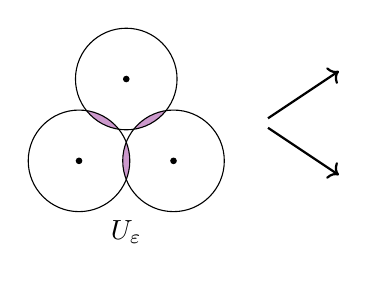
\begin{tikzpicture}[scale=0.6]
  \def\r{1.075}
  \coordinate (A) at (0,0);
  \coordinate (B) at (2,0);
  \coordinate (C) at (1,{sqrt(3)});

  % Intersecciones violetas
  \begin{scope}
    \clip (A) circle (\r);
    \fill[violet!40] (B) circle (\r);
  \end{scope}
  \begin{scope}
    \clip (B) circle (\r);
    \fill[violet!40] (C) circle (\r);
  \end{scope}
  \begin{scope}
    \clip (A) circle (\r);
    \fill[violet!40] (C) circle (\r);
  \end{scope}

  % Puntos
  \fill (A) circle (2pt);
  \fill (B) circle (2pt);
  \fill (C) circle (2pt);

  % Bordes de los círculos
  \draw (A) circle (\r);
  \draw (B) circle (\r);
  \draw (C) circle (\r);

  % Flechas hacia los complejos (relativas a esta subfigura)
  \draw[->, thick] (4.0,0.9) -- ++(1.5,1.0);  % Čech
  \draw[->, thick] (4.0,0.7) -- ++(1.5,-1.0); % Vietoris–Rips

  % Etiqueta
  \node at (1,-1.5) {$U_\varepsilon$};
\end{tikzpicture}
\end{subfigure}
\hfill
% ------------------- Subfigura 3: Complejos -------------------
\begin{subfigure}{0.3\textwidth}
\centering
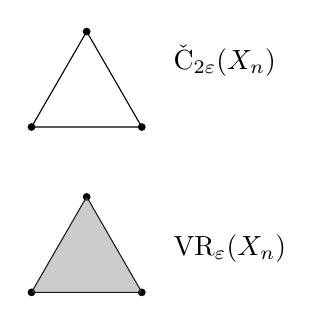
\begin{tikzpicture}[scale=0.7]
  % Complejo de Čech (arriba)
  \begin{scope}[shift={(0,1.5)}]
    \coordinate (C1) at (0,0);
    \coordinate (C2) at (2,0);
    \coordinate (C3) at (1,{sqrt(3)});
    \fill (C1) circle (2pt);
    \fill (C2) circle (2pt);
    \fill (C3) circle (2pt);
    \draw (C1) -- (C2) -- (C3) -- cycle;
    \node[right] at (2.4,1.2) {$\check{\operatorname{C}}_{2\varepsilon}(X_n)$};
  \end{scope}

  % Complejo de Vietoris–Rips (abajo)
  \begin{scope}[shift={(0,-1.5)}]
    \coordinate (V1) at (0,0);
    \coordinate (V2) at (2,0);
    \coordinate (V3) at (1,{sqrt(3)});
    \fill (V1) circle (2pt);
    \fill (V2) circle (2pt);
    \fill (V3) circle (2pt);
    \draw (V1) -- (V2) -- (V3) -- cycle;
    \fill[gray, opacity=0.4] (V1) -- (V2) -- (V3) -- cycle;
    \node[right] at (2.4,0.8) {$\operatorname{VR}_{\varepsilon}(X_n)$};
  \end{scope}
\end{tikzpicture}
\end{subfigure}
\end{figure}
Notar que, como $Č_{2 \varepsilon}(X_n)$ es el nervio del cubrimiento $\{B_\varepsilon(x)\}_{x \in X_n}$, por el teorema del nervio resulta homotópicamente equivalente a $\displaystyle \bigcup_{x \in X_n} B_\varepsilon(x)$.
\\
\\
Valen, además, las siguientes inclusiones:
\[
VR_\varepsilon \hookrightarrow Č_{\varepsilon\sqrt{2}} \hookrightarrow VR_{\varepsilon\sqrt{2}}
\]
Por lo tanto, cualquier propiedad topológica que persista bajo $VR_{\varepsilon'} \hookrightarrow VR_{\varepsilon}$ es también una propiedad de $Č_{\varepsilon'}$ si $\sqrt{2}\varepsilon'< \varepsilon$ pues
\[
VR_{\varepsilon'} \hookrightarrow Č_{\varepsilon' \sqrt{2}} \hookrightarrow Č_\varepsilon \hookrightarrow VR_\varepsilon
\]
\subsection{Módulos intervalo y barcodes}
\begin{definition}
Dados $i \leq j \in \mathbb{Z}$ y un módulo de persistencia $(V_i, \phi_i)_i$, se define su \textit{grupo de homología persistente asociado} como $\text{im}\phi^{i \rightarrow j} \subseteq V_j$.
\end{definition}
Para cada $k$, el grupo de homología persistente asociado al módulo de persistencia consiste en las clases $H_k(V_i)$ que al incluirlas en $H_k(V_j)$ son no triviales.
\begin{definition}
Sean $i < j \in \mathbb{Z}_{\geq0} \cup \{\infty\}$. Definimos el \textit{módulo intervalo} $(I_k^{[i,j)})_k$ como el módulo de persistencia $(I_k^{[i,j)}, \psi_k)_k$ donde
\[
I_k^{[i,j)} = 
\begin{cases}
  \mathbb{F} & \text{si } i \leq k < j \\
  0 & \text{si no}
\end{cases}
\]
y cuya estructura lineal está dada por las funciones $\psi_k: I_k^{[i,j)} \rightarrow I_{k+1}^{[i,j)}$ donde
\[
\psi_k = 
\begin{cases}
  id_{\mathbb{F}} & \text{si } i \leq k < j \\
  0 & \text{si no}
\end{cases}
\]
Es decir,
\[
\ldots \xrightarrow{0} 0 \xrightarrow{0} \mathbb{F} \xrightarrow{\psi_i} \mathbb{F} \xrightarrow{\psi_{i+1}} \ldots \xrightarrow{\psi_{j-2}} \mathbb{F} \xrightarrow{\psi_{j-1}} 0 \xrightarrow{0} \ldots 
\]
\end{definition}
El \textit{teorema de estructura para módulos de persistencia} nos asegura que podemos obtener una descomposición de nuestro módulo de persistencia en módulos intervalo.
\begin{definition}
    Un módulo de persistencia $(V_k, \phi_k)_k$ es \textit{de tipo finito} si $\dim V_k < \infty$ para todo $k$ y existe un $k_0$ tal que $\phi_k$ es un isomorfismo si $k \geq k_0$.
\end{definition}
\begin{theorem}[Teorema de estructura para módulos de persistencia]
    \\
    Dado $(V_k, \phi_k)_k$ un módulo de persistencia de tipo finito, existen $BC(V_k, \phi_k)_k$ un conjunto finito de intervalos $[i,j)$ donde $0 \leq i \leq j \leq \infty$ y una función de multiplicidad $\mu: BC(V_k, \phi_k)_k \rightarrow \mathbb{N}$ tales que
    \[
    (V_k, \phi_k)_k \simeq \bigoplus_{[i,j) \in BC(V_k, \phi_k)_k} (I_k^{[i,j)})_k^{\mu[i,j)}
    \]
\end{theorem}
Es decir que, para cada momento $k$, $V_k$ es la suma directa de todos los intervalos que ``están vivos en $k$''.
\begin{proof}
Sea $(V_k, \phi_k)_k$ un módulo de persistencia de tipo finito.
\\
\\
Definamos $\displaystyle V \coloneqq \bigoplus_k V_k$ y una acción $t$ en $V$ tal que $t|_{V_k} \coloneqq \phi_{k+1}$. De esta forma, le damos a $V$ una estructura de $\mathbb{F}(t)$-módulo graduado de tipo finito sobre el anillo graduado $\mathbb{F}(t)$.
\\
\\
Así que estamos en condiciones de aplicar el teorema de estructura de módulos graduados de tipo finito sobre un dominio de ideales principales, que nos dice que podemos descomponer a $V$ de manera única -salvo isomorfismos- como $V \simeq L \oplus T$, donde $L$ es libre y $T$ de torsión.
\\
Es decir, 
\[
L = \bigoplus_{i} \, (t^i\mathbb{F}(t))^{\mu_i}, \qquad T = \bigoplus_{[i,j)} (\frac{t^i\mathbb{F}(t)}{t^j})^{\mu_{i,j}}
\]
Luego L induce los intervalos $(I_k^{[i,+\infty)})_k$ y T los intervalos $(I_k^{[i,j)})_k$.
\end{proof}
Al conjunto $BC(V_k,\phi_k)_k$ junto a las multiplicidades lo llamamos el \textit{barcode de $(V_k, \phi_k)_k$}, que resulta una descomposición única -salvo isomorfismos de módulos de persistencia-.
\\
\\
\\
Supongamos que queremos calcular el barcode del complejo simplicial $K$, cuyos vértices $\{x_0, x_1, \ldots, x_{l}\}$ son equidistantes -a distancia $2\delta$- sobre $S^1$.
\\
\\
Construimos la filtración $\{U_\varepsilon: \varepsilon \in [0, 1)\}$:
\\
\begin{figure}[H]
\centering
% --- Solo puntos
\begin{subfigure}{0.2\textwidth}
\centering
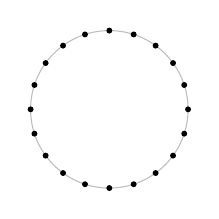
\begin{tikzpicture}[scale=1]
  \draw[gray!50] (0,0) circle(1);
  \foreach \i in {0,...,19} {
    \filldraw (360/20*\i:1) circle(0.03);
  }
\end{tikzpicture}
\caption*{$\varepsilon=0$}
\end{subfigure}\hfill
% --- epsilon < delta
\begin{subfigure}{0.2\textwidth}
\centering
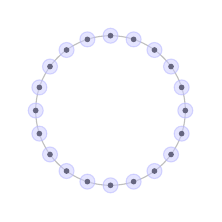
\begin{tikzpicture}[scale=0.95]
  \draw[gray!50] (0,0) circle(1);
  \foreach \i in {0,...,19} {
    \filldraw (360/20*\i:1) circle(0.03);
    \draw[blue!30,fill=blue!20,opacity=0.5] (360/20*\i:1) circle(0.1);
  }
\end{tikzpicture}
\caption*{$\varepsilon<\delta$}
\end{subfigure}\hfill
% --- epsilon >= delta
\begin{subfigure}{0.2\textwidth}
\centering
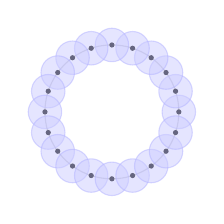
\begin{tikzpicture}[scale=0.85]
  \draw[gray!50] (0,0) circle(1);
  \foreach \i in {0,...,19} {
    \filldraw (360/20*\i:1) circle(0.03);
    \draw[blue!30,fill=blue!20,opacity=0.5] (360/20*\i:1) circle(0.25);
  }
\end{tikzpicture}
\caption*{$\varepsilon \geq \delta$}
\end{subfigure}\hfill
% --- epsilon <= 1 - ~epsilon
\begin{subfigure}{0.2\textwidth}
\centering
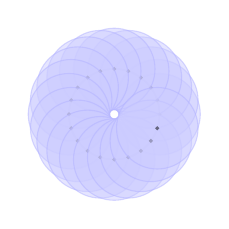
\begin{tikzpicture}[scale=0.575]
  \draw[gray!50] (0,0) circle(1);
  \foreach \i in {0,...,19} {
    \filldraw (360/20*\i:1) circle(0.03);
    \draw[blue!30,fill=blue!20,opacity=0.5] (360/20*\i:1) circle(0.9);
  }
\end{tikzpicture}
\caption*{$\varepsilon \leq 1-\tilde{\varepsilon}$}
\end{subfigure}\hfill
% --- epsilon = 1
\begin{subfigure}{0.2\textwidth}
\centering
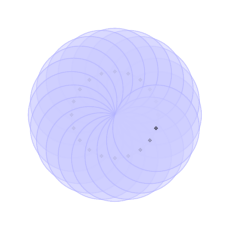
\begin{tikzpicture}[scale=0.55]
  \draw[gray!50] (0,0) circle(1);
  \foreach \i in {0,...,19} {
    \filldraw (360/20*\i:1) circle(0.03);
    \draw[blue!30,fill=blue!20,opacity=0.5] (360/20*\i:1) circle(1);
  }
\end{tikzpicture}
\caption*{$\varepsilon=1$}
\end{subfigure}
\end{figure}
La componente arco-conexa representada por $[x_0]$ nace en $\varepsilon=0$ y muere en $+\infty$. Las representadas por $[x_i - x_0]_{i>0}^{i=l}$ nacen en $\varepsilon=0$ y mueren en $\varepsilon = \delta$, pues a partir de ese radio todos los puntos pertenecen a la misma componente.
\\
\\
El ciclo representado por $[x_0 x_1] + [x_1 x_2] + \ldots + [x_{l-1} x_l] + [x_l x_0]$ nace en $\varepsilon \geq \delta$ y muere en $\varepsilon = 1$.
\\
\\
Como para cada $n$ tenemos un módulo de persistencia correspondiente a $H_n$, podemos aplicar el teorema para calcular su descomposición: para $H_0$ tenemos un módulo intervalo $I[0, +\infty)$ con multiplicidad $\mu_{[0, +\infty)} = 1$ y uno $I[0,\delta)$ con multiplicidad $\mu_{[0,\delta)} = l$. Para $H_1$, tenemos $I^{[\delta, 1)}$ con multiplicidad $\mu_{[\delta, 1)} = 1$.
\\
\\
Así,
\[
H_0(K, \mathbb{F}) \simeq I[0, +\infty)^1 \oplus I[0,\delta)^l
\]
\[
H_1(K, \mathbb{F}) \simeq I[\delta, 1)^1
\]
Es decir,
\[
H_0(K, \mathbb{F}) \simeq \mathbb{F}^{l+1} \rightarrow \ldots \rightarrow \mathbb{F}^{l+1} \xrightarrow{\psi_{\delta}} \mathbb{F} \rightarrow \ldots \xrightarrow{\psi_1} \mathbb{F}
\]
\[
H_1(K, \mathbb{F}) \simeq 0 \rightarrow \ldots \rightarrow \mathbb{F} \xrightarrow{\psi_{\delta}} \mathbb{F} \rightarrow \ldots \xrightarrow{} \mathbb{F} \xrightarrow{\psi_1} 0
\]
Y el barcode de nuestra filtración es
\begin{center}
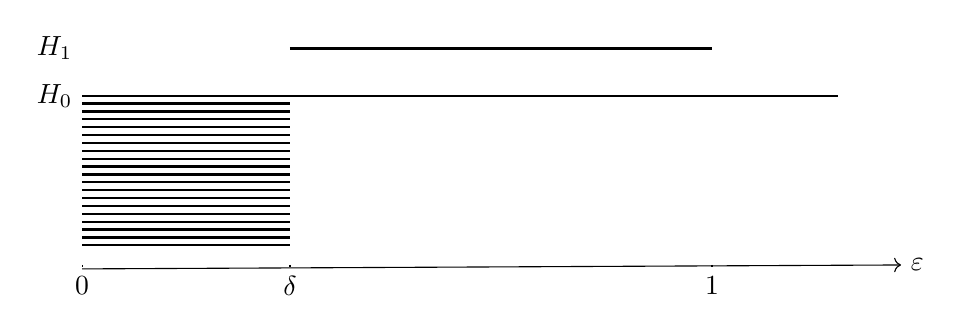
\begin{tikzpicture}[xscale=8, yscale=-0.5]
% H_1 label
\node[left] at (0,0) {$H_1$};

% H_1 barra
\draw[thick] (0.33, 0) -- (1, 0); % [δ, 1)

% H_0 label
\node[left] at (0,1.2) {$H_0$};

% H_0 barras
\draw[thick] (0, 1.2) -- (1.2, 1.2);   % [0, ∞)
\foreach \i in {1,...,19} { % 19 barras cortas de 0 a δ
  \draw[thick] (0, {1.2+0.2*\i}) -- (0.33, {1.2+0.2*\i});
}

% Ejes
\draw[->] (0,5.6) -- (1.3,5.5) node[right] {$\varepsilon$};
\draw (0,5.5) -- (0,5.55) node[below] {$0$};
\draw (0.33,5.5) -- (0.33,5.55) node[below] {$\delta$};
\draw (1,5.5) -- (1,5.55) node[below] {$1$};

\end{tikzpicture}
\end{center}
\subsubsection{Estabilidad de barcodes}
Como estamos trabajando con muestras, necesitamos que los \textit{barcodes} de módulos de persistencia sean estables: que dados dos espacios ``parecidos'', sus barcodes también lo sean.
\begin{definition}
    Sean $B$ y $B'$ multiconjuntos de intervalos en $\mathbb{R} \cup \{+\infty\}$. Para $\varepsilon \geq 0$ definimos un $\bm\delta$-matching entre $B$ y $B'$ como una biyección $\gamma: B_0 \xrightarrow{\simeq} B_0'$ para subconjuntos $B_0 \subseteq B$, $B_0' \subseteq B'$ tales que:
    \[
    \gamma([s,t)) = [s',t') \Rightarrow \lvert s-s' \rvert, \, \lvert t-t' \rvert \leq \delta,
    \]
    \[
    [s,t) \in B \setminus B_0 \, \cup \, B' \setminus B_0' \Rightarrow t-s \leq 2\delta
    \]
\end{definition}
\begin{definition}
    Definimos la distancia bottleneck entre $B$ y $B'$ como
    \[
    d_{bot}(B,B') \coloneqq \inf\{\delta \geq 0 : \text{existe un }\delta \text{-matching entre $B$ y $B'$}\}
    \]
\end{definition}
\begin{definition}
    Sea $(X, d_X)$ un espacio métrico. Para $\varepsilon \geq 0$, definimos el engordado de $X$ como $\displaystyle X_\varepsilon \coloneqq \bigcup_{x \in X} B_\varepsilon(x)$
\end{definition}
\begin{definition}
    Sean $(X, d_X), (Y, d_Y)$ espacios métricos con $X, Y \subseteq \mathbb{R}^n$. La distancia de Hausdorff entre $X$ e $Y$ es:
    \[
    d_H(X, Y) \coloneqq \inf \{\varepsilon \geq 0 : X \subseteq Y_\varepsilon, Y \subseteq X_\varepsilon \}
    \]
\end{definition}

El \textit{teorema de estabilidad generalizado} nos asegura que los barcodes de filtraciones asociadas a espacios que están cerca también lo están:
\begin{theorem}[Teorema de estabilidad generalizado]
\\
Sean $(X,d_X)$, $(Y, d_Y)$ espacios métricos compactos. Entonces:
    \[
    d_{bot}(BC(VR(X_n)),BC(VR(X))) \leq 2d_H(X_n,X)
    \]
\end{theorem}

Esto quiere decir que, si la muestra del espacio es ``buena'', la estimación de su homología también lo será. Necesitamos entonces resultados que nos aseguren cuándo nuestra muestra lo es:
\begin{definition}
    Dado $X \subseteq \mathbb{R}^m$, definimos el $reach(X) = \displaystyle \inf_{z \in \text{Med}(X)} d(z, X)$, donde $\text{Med}(X)$ es su eje medial.
\end{definition}

\begin{proposition}
    Sea $X$ una subvariedad compacta de $\mathbb{R}^m$, $\{X_n\}_n$ una muestra aleatoria independiente e idénticamente distribuida respecto de la probabilidad uniforme de $X$. Si $\delta>0$ y $\varepsilon < \text{reach}(X)/2$, entonces $n$ ``suficientemente grande'' implica que $d_H(X_n, X) < \varepsilon/2$ con probabilidad mayor a $1 - \delta$.
\end{proposition}
El \textit{teorema de Niyogi, Smale y Weinberger} nos asegura que, bajo ciertas hipótesis, la homología de $X_\varepsilon$ coincide con la de $X$ (es decir, la distancia entre sus barcodes es chica):
\begin{theorem}[Teorema de Niyogi, Smale y Weinberger]
\\
Sea $X$ una subvariedad compacta de $\mathbb{R}^m$ y supongamos que los puntos de $X_n$ están distribuidos independiente e idénticamente según la probabilidad uniforme de $X$.
\\
Entonces, existen un número $\alpha_X$ y constantes $\beta_1(X, \alpha_X)$ y $\beta_2(X, \alpha_X)$ tales que, si $0 < \varepsilon < 1/2.\alpha_X$, dado $\delta > 0$, la homología de $X_{\varepsilon}$ coincide con la de $X$ con probabilidad mayor a $1 - \delta$ para $n > \beta_1(\log(\beta_2) + \log(1/\delta))$.
\end{theorem}
Esto quiere decir que, para una muestra lo suficientemente grande, existe un intervalo para el cual nuestro $\varepsilon$ es el que necesitamos, lo que respalda el enfoque de estudiar características persistentes.
\\
\\
\\
\section{Cycling signatures}
Ahora sí, estamos en condiciones de adentrarnos en el análisis de las cycling signatures.
\\
\\
Supongamos que tenemos un sistema dinámico continuo dado por $\Phi : \mathbb{R} \times X \rightarrow X$ en el espacio de fases $X \subseteq \mathbb{R}^d$, y que queremos calcular sus órbitas periódicas.
\\
\\
Vamos a considerar a las órbitas periódicas como ``trayectorias cerradas que tienen la topología de un círculo''. Dado un segmento $\gamma = \Phi([a,b],x) \subseteq X$, decimos que $\gamma$ contiene una órbita periódica si y sólo si ``es un círculo'', es decir, si $H_1(\gamma) \neq 0$.
\\
\\
Notar que, por un lado, no tenemos $\Phi$ sino un conjunto de datos pertenecientes al sistema, por lo que cualquier segmento $\gamma = (x_k,x_{k+1},...,x_l)$ es finito y por lo tanto $H_1(\gamma)=0$. Además, dado que el sampleo del sistema puede haber estado expuesto a ruido, un segmento periódico puede haber sido perturbado en uno ``casi periódico''. Por el otro, sólo considerar información espacial no parece ser suficiente para distinguir características topológicas u homológicas de una serie de tiempo.
\\
\\
Para sortear estos problemas, consideraremos \textit{thickenings} de $\gamma$ en el espacio tangente.
\subsection{Espacio tangente y \textit{r}-thickenings}
\begin{definition}
    Dado $r \geq 0$ y $A$ un subconjunto de un espacio métrico $(X,d_X)$, definimos el r-thickening de $A$ como $O_r(A) = \{ x \in X : d_X(x,A) < r \}$.
\end{definition}
\begin{definition}
    Dado $X \subseteq \mathbb{R}^d$, definimos su espacio tangente $T(X) = \{(x,v) \in X \times \mathbb{R}^d : v \text{ es el vector tangente de } x\}$.
\end{definition}
Notar que el espacio tangente nos permite recuperar, además de la espacial, la información direccional del conjunto. Y como sólo nos interesa la dirección de $v$ y no su rapidez, podemos normalizar los vectores y pasar al \textit{espacio tangente unitario}.
\begin{definition}
    Dado $X \subseteq \mathbb{R}^d$, definimos su espacio tangente unitario $UT(X) = \{ (x,v) \in T(X) : \|v\|_2 = 1 \} = X \times S^{d-1}_2$
\end{definition}
Para pasar al espacio tangente unitario, queremos normalizar los vectores del espacio tangente que sean, obviamente, no nulos. A tal fin, consideramos $X_0$ el conjunto de puntos de $X$ cuyo vector tangente se anula. Definimos la sección
\[
    \rho : X \setminus X_0 \to UT(X \setminus X_0), \quad x \mapsto (x, v(x)/\|v(x)\|_2 )
\]
y la serie de tiempo
\[
    \rho(\Gamma) := \left\{ \rho(x_0), \dots, \rho(x_N) \right\}
\]
Así, si $\gamma$ es un subsegmento de nuestra serie de tiempo $\Gamma$, queremos entender la dinámica de recurrencia de $\rho(\gamma)$ vista en $UT(X)$. La métrica que nos permitirá construir los thickenings en el $UT(X)$ la definiremos como
\[
    d_C((x,v),(z,w)) \coloneqq \max\left\{ \|x-z\|_2, C \|v-w\|_2 \right\}
\]
para cierto $C > 0$ \textit{adecuado}.
\\
\\
En la siguiente sección definiremos el \textit{espacio de comparación}, que será el espacio en el que miraremos a nuestra serie de tiempo.
\subsection{El espacio de comparación y el espacio de comparación cúbico}
Queremos construir un espacio en el que tenga sentido ``mirar'' a nuestra serie de tiempo. Definimos, entonces, el \textit{espacio de comparación} de la siguiente manera:
\begin{definition}
    Un espacio de comparación para una serie de tiempo $\Gamma \subseteq X$ es un entorno de $\rho(\Gamma) \subseteq UT(X)$. Lo notamos $Y$.
\end{definition}
Sin embargo, queremos un espacio que además de recuperar la dinámica del sistema sea sencillo de computar. Como $S_\infty$ es más fácil de computar que $S_2$, y tenemos un homeomorfismo
\[
    \eta : UT_2(\mathbb{R}^d) \rightarrow UT_\infty(\mathbb{R}^d), \quad (p,v) \mapsto (p,v/\|v\|_\infty)
\]
podemos considerar el espacio tangente unitario pero con respecto a la norma $l_\infty$. Es decir,
\[
    UT_\infty(\mathbb{R}^d) = \{(p,v) \in T(\mathbb{R}^d): \|v\|_\infty = 1 \}
\]

Notar que podemos obtener un espacio de comparación $Y$ definiendo un entorno $U$ de $\eta(\rho(\Gamma))$ y tomando $Y = \eta^{-1}(U)$.
\\
\\
Ahora bien, para construir nuestro \textit{espacio de comparación cúbico} -es decir, nuestro espacio de comparación fácilmente computable-, vamos a considerar la intersección entre el espacio tangente unitario (con respecto a la norma infinito) y un entorno de nuestra serie de tiempo. A tal fin, dados $p \in \mathbb{R}^d$ y $n \in \mathbb{R}_{>0}$ definimos
\[
    Q_n(p) = \prod_{i=1}^d [p_i - n/2, p_i +n/2]
\]
Para cada $r, k \in \mathbb{R}_{>0}$, $p \in r.\mathbb{Z}^d$ y $q \in 1/k.\mathbb{Z}^d$, definimos
\[
    Q_{r,k}(p,q) = Q_r(p) \times Q_{1/k}(q) \subseteq T(\mathbb{R}^d)
\]

Notar que la colección de estas cajas cubre todo $\mathbb{R}^{2d} = T(\mathbb{R}^d)$. Para cubrir el espacio tangente unitario, fijamos los parámetros $r \in \mathbb{R}_{>0}$ y $k \in \mathbb{N}_{>0}$ y consideramos
\[
    \mathcal{Q}^d_{r,k} = \{Q_{r,k}(p,q) : p \in r\mathbb{Z}^d, q \in k\mathbb{Z}^d, \|q\|_\infty = 1 \}
\]

Dado $\varepsilon > 0$, el conjunto $O_\varepsilon(\eta(\rho(\Gamma)))$ es un entorno de nuestra serie de tiempo vista en el espacio tangente unitario. Podemos entonces definir al espacio de comparación cúbico para que cubra un entorno de $\eta(\rho(\Gamma))$ de la siguiente manera:
\[
    Y_\infty \coloneqq \{Q \in \mathcal{Q}^d_{r,k} : Q \cap O_\varepsilon(\eta(\rho(\Gamma))) \neq \emptyset \} \subseteq T_{\infty}(\mathbb{R}^d)
\]

Notamos $|Y_\infty|$ a la unión de todas las cajitas en $Y_\infty$, es decir, $\displaystyle |Y_\infty| = \bigcup_Q \{ Q \in Y_\infty \}$. Si quisiéramos recuperar el espacio de comparación a partir del espacio de comparación cúbico, tomamos $\eta^{-1}(p_\infty(|Y_\infty|))$, donde
\[
p_\infty: T(\mathbb{R}^d) \setminus(\mathbb{R}^d \times \{0\}) \rightarrow UT_\infty(\mathbb{R}^d), \quad (p,v) \mapsto (p, v/\|v\|_\infty)
\]

Ahora sí, estamos en condiciones de definirlo.
\begin{definition}
    Un \textit{espacio de comparación cúbico} es un conjunto $Y_\infty \subseteq \mathcal{Q}^d_{r,k}$ para ciertos $r \in \mathbb{R}_{>0}$ y $k \in \mathbb{N}$ tal que $Y = \eta^{-1}(p_\infty(|Y_\infty|))$ es un espacio de comparación para $\Gamma \subseteq \mathbb{R}^d$.
\end{definition}
En la siguiente sección construiremos formalmente las cycling signatures.
\subsection{Construyendo las cycling signatures}
Recordemos que no sólo queremos identificar subsegmentos periódicos, sino que además queremos poder compararlos cualitativamente. Esto nos permitirá identificar distintos \textit{tipos} de órbitas periódicas en el sistema.
\\
\\
En primer lugar, notemos que, como $Y$ es un entorno de $\rho(\Gamma)$, existe un $r_0 = r_0(Y) > 0$ tal que para cualquier $\gamma \in \Gamma$, si $r < r_0$ tenemos la inclusión
\[
    i_\gamma,_r : {O_r}(\rho(\gamma))) \hookrightarrow Y
\]
donde el \textit{r-thickening} lo tomamos con respecto a la métrica $d_C$ en el $UT(X)$.
\\
\\
Esta inclusión induce en la homología el morfismo
\[
    H_1(i_\gamma,_r): H_1({O_r}(\rho(\gamma))) \hookrightarrow H_1(Y)
\]

Como $H_1(i_\gamma,_r)$ es un morfismo, $\text{im}(H_1(i_\gamma,_r))$ es un subespacio de $H_1(Y)$. Tiene sentido, entonces, distinguir segmentos cíclicos según los subespacios que inducen en el espacio vectorial $H_1(Y)$.
\begin{definition}
    Un subsegmento $\gamma$ es \textit{r-cíclico} si $H_1({O_r}(\rho(\gamma))) \neq 0$.
\end{definition}
\begin{definition}
    Definimos el espacio r-cíclico de un subsegmento $\gamma$ como
    \[
        \text{Cyc}_r(\gamma,Y) := \text{im}H_1(i_\gamma,_r)
    \]
    y el \textit{r-rango} como $\dim (\text{Cyc}_r(\gamma,Y))$.
\end{definition}
Como queremos estudiar órbitas periódicas, centraremos el análisis en los subsegmentos $\gamma$ de \textit{r-rango} 1.
\\
\\
Notar que la elección del radio de thickening es crucial en la construcción de los espacios, pero no es evidente. Utilizaremos, entonces, el enfoque de homología persistente y analizaremos ``todos'' los posibles radios. Esto tiene sentido puesto que, si $\gamma$ es un subsegmento de una serie de tiempo $\Gamma$, la familia de \textit{r}-thickenings $O(\rho(\gamma)) \coloneqq (O_r(\rho(\gamma)))_{r \in I}$ es una filtración de espacios topológicos. Para definir la \textit{cycling signature}, construiremos filtraciones tanto para nuestro subsegmento en cuestión como para el espacio de comparación.
\\

Sea $Y$ un espacio de comparación para $\Gamma$. Para cada $r \in I$, definimos $\triangle Y_r = Y$ y consideramos $\triangle Y = (\triangle Y_r)_{r \in I}$ la filtración constante de $Y$, que por supuesto es una filtración de espacios topológicos. Si definimos $I = [0,r_0)$ para el $r_0$ obtenido previamente, para cada $r \in I$ tenemos la inclusión
\[
    i_\gamma,_r : {O_r}(\rho(\gamma))) \hookrightarrow Y
\]
a partir de la cual obtenemos una colección de inclusiones $(i_{\gamma,r})_{r \in I}$, y por lo tanto un morfismo
\[
    i_\gamma : O(\rho(\gamma)) \hookrightarrow \triangle Y
\]
entre filtraciones de espacios topológicos indexados en $I$ tal que el siguiente diagrama conmuta:
\[
\begin{tikzcd}
O_r(\rho(\gamma)) \arrow[r, hookrightarrow, "i_{\gamma, r}"] \arrow[d, hookrightarrow, "O_{r,s}"'] & \triangle Y_r=Y \arrow[d, equal] \\
O_s(\rho(\gamma)) \arrow[r, hookrightarrow, "i_{\gamma, s}"] & \triangle Y_s=Y
\end{tikzcd}
\]
Pasando a la homología, que nos permite pasar de espacios topológicos a espacios vectoriales, se induce un morfismo
\[
H_1(i_\gamma) : H_1({O}(\rho(\gamma))) \hookrightarrow H_1(\triangle Y)
\]
de módulos de persistencia. Y por lo tanto $\text{im}(H_1(i_\gamma))$ resulta una filtración de espacios vectoriales.
\\
\\
Estamos en condiciones, entonces, de dar la definición de cycling signature:
\begin{definition}
    Dado un subsegmento $\gamma \in \Gamma$ y un espacio de comparación $Y$, definimos a la cycling signature $Cyc(\gamma, Y)$ como la filtración de espacios vectoriales $\text{im}(H_1(i_\gamma)) \leq H_1(\triangle Y)$.
\end{definition}
Es claro que lo que quisiéramos es poder calcular la imagen del morfismo $H_1(i_\gamma)$. Sin embargo, como ya sabemos que eso es difícil computacionalmente, vamos a usar complejos simpliciales para discretizar los \textit{r}-thickenings de los subsegmentos, y los espacios de comparación cúbicos para construir los espacios de comparación correspondientes.
\\
\\
Para $Y = \eta^{-1}(p_\infty(|Y_\infty|))$, por \cite{cycling-sigs} sabemos que el siguiente diagrama
\[
\begin{tikzcd}
    H_1(O(\rho(\gamma))) \arrow[r, "H_1(i_{\gamma})"] & H_1(\triangle Y) \arrow[d, "\simeq"'] 
    \\
    H_1(\check{C}(\rho(\gamma))) \arrow[u, "\simeq"'] \arrow[r, "H_1(\phi)"'] & H_1(\triangle Y_\infty)
\end{tikzcd}
\]
es conmutativo. Y por lo tanto nos basta con entender cómo calcular la base del morfismo $\operatorname{im}H_1(\phi)$, que es lo que veremos en el siguiente capítulo.
\newpage
\section{Algoritmo e implementación}
Como $H_1(\phi)$ es un morfismo entre módulos de persistencia y $H_1(\triangle Y_\infty)$ es una filtración de espacios vectoriales, por lo demostrado anteriormente sabemos que entonces $\text{im}(H_1(\phi))$ también es una filtración de espacios vectoriales y que podemos restringirnos a calcular la imagen de la parte inmortal del complejo. Es decir, queremos calcular la imagen del morfismo $H_1(\phi)|_{H_1(Č(\rho(\gamma)))^\infty}$, para lo cual utilizaremos reducción de matrices, como muestra la siguiente proposición:
\begin{proposition}
    Sea $\phi: V \rightarrow W$ un morfismo entre filtraciones de espacios vectoriales. Sean $B^V = \{v_1,...,v_n\}$ base de $V$ y $B^{W^*} = \{\alpha_1,...,\alpha_m\}$ base de $W^*$, el espacio dual de $W$. Una base para $\text{im}\phi$ se puede computar reduciendo la matriz $M = [\alpha_i(\phi(v_j))]_{i,j}$.
\end{proposition}
Así, dado un espacio de comparación cúbico $Y_\infty$, para computar $\text{Cyc}(\gamma, Y_\infty)$ necesitamos reducir la matriz $M_{i,j} = [\alpha_i(\phi(v_j))]_{i,j}$ donde los $\alpha_i$ son una base de $H_1(\triangle Y_\infty)$ y los $v_j$ son una base de $H_1(\check{\text{C}}(\rho(\gamma)))$. Sin embargo, dada la diferencia en el costo computacional, es común utilizar los complejos de Vietoris-Rips en lugar de los de Čech a la hora de realizar los cálculos. Por lo que para computar los $v_j$, computamos el barcode $(b_i, d_i)_i$ y los generadores $G=(g_i)_i$ de $H_1(\operatorname{VR}(\rho(\gamma)))$. Para computar los $\alpha_i$, aplicamos el algoritmo de correducción.
\\
\\
\\
No hay que olvidar mencionar que este cálculo requiere elegir varios parámetros: la métrica $d_C$ -y conocer el radio máximo de filtración $r_0$- para poder construir los thickenings, y $r \in \mathbb{R}_{>0}$ y $k \in \mathbb{N}$ para definir el espacio de comparación cúbico $Y_\infty \subseteq \mathcal{Q}_{r,k}$.
\\
\\
Según los autores del paper, la idea es que $r$ controla la resolución espacial, y se elige de acuerdo a la escala típica de la dinámica, y $k$ controla la resolución angular, y se elige según cuánta sensibilidad a la dirección se necesita. Teniendo $r$ y $k$, su propuesta es definir $C = r.k$ y $r_0 = r$.
\newpage
\section{Experimentos}
En el siguiente apartado analizaremos los resultados obtenidos de los experimentos realizados en el paper para calcular las cycling signatures de los atractores de Double-Well y Lorenz. 
\\
\\
Pero antes, veamos la importancia del radio de thickening, el espacio tangente y el espacio de comparación, usando como ejemplo el atractor de Double-Well.
\\
\\
\subsection{La importancia del radio de thickening y el espacio tangente, descripción gráfica}
En primer lugar, supongamos que estamos analizando el siguiente subsegmento perteneciente a la serie de tiempo del atractor de double-well:
\\
\begin{figure}[H]
    \centering
    \includegraphics[width=0.5\linewidth]{segmentsDifferentR-doubleWell_paper.png}
\end{figure}
Es claro que $r$ pequeños nos llevan a subsegmentos de rango 0, mientras que $r$ más grandes nos llevan a rango 1. Con el $r$ de la figura izquierda, no detectaríamos ese subsegmento como periódico. Pero con el $r$ de la derecha, sí.
\\
\\
En particular, hay un umbral $\overline{r}$ tal que
\[
\text{dim}(\text{Cyc}_r(\gamma,Y)) = 
\begin{cases}
    0 & \text{si } r < \overline{r} \\
    1 & \text{si } \overline{r} < r < r_0(Y)
\end{cases}
\]
En segundo lugar, supongamos que estamos analizando una elipse $E = \{x \in \mathbb{R}^2 : (x_1/a)^2 + (x_2/b)^2 = 1\}$, con $b < a$. En $\mathbb{R}^2$ con la métrica inducida por la norma euclídea, tenemos que
\[
H_1(O_r(E)) =
\begin{cases}
\mathbb{F} & \text{si } 0 \leq r < b \\
0  & \text{en otro caso}
\end{cases}
\]
Notar que, aún habiendo considerado un objeto que es una órbita periódica en sí, si $b$ es mucho más chico que $a$ sólo $r$-s muy pequeños conducen a $H_1$ no trivial. Esto es un problema si pasamos a una muestra de una serie de tiempo de la elipse, pues podríamos no sólo no ser capaces de distinguir características relevantes homológicamente, sino también haber introducido algunas al generar la muestra.
\\
\\
Lo que quisiéramos es detectar un solo ciclo, que corresponde al segmento formado por todos los puntos de la muestra. Sin embargo, al observar la siguiente figura puede verse que muchos segmentos $\gamma$ obtenidos de la muestra de la elipse parecen cumplir con el criterio $H_1(O_r(\gamma)) \neq 0$. Por ejemplo, hubiéramos erróneamente detectado el segmento marcado en azul oscuro como un ciclo.
\begin{figure}[H]
    \centering
    \begin{subfigure}[t]{0.4\linewidth}
        \centering
        \includegraphics[width=\linewidth]{elipseExample_paper.png}
    \end{subfigure}
    \begin{subfigure}[t]{0.4\linewidth}
        \centering
        \includegraphics[width=\linewidth]{elipseExample.png}
    \end{subfigure}
\end{figure}
Si pasamos al espacio tangente, recuperamos la dinámica natural de los segmentos, porque la distancia entre dos puntos consecutivos resulta siempre más chica que la de dos puntos opuestos en la elipse.
\begin{figure}[H]
    \centering
    \includegraphics[width=0.4\linewidth]{elipseWithVelocitiesExample_paper.png}
\end{figure}
\subsection{La métrica $d_C$ en el espacio de comparación}
Como motivación, observemos primero la serie de tiempo del atractor de double-well con sus vectores tangentes:
\begin{figure}[H]
    \centering
    \includegraphics[width=0.5\linewidth]{tangentField-doubleWell.png}
\end{figure}
en donde se pueden ver dos agujeros bien marcados y se puede vislumbrar un tercero en el centro de la figura.
\\
\\
Si ignoramos el espacio tangente unitario (es decir, definimos $C = 0$ en nuestra métrica $d_C$), obtenemos el siguiente gráfico del espacio de comparación:
\begin{figure}[H]
    \centering
    \includegraphics[width=0.5\linewidth]{simplifiedComparisonSpace-doubleWell_paper.png}
\end{figure}
La serie de tiempo está cubierta por cajas grises, cuya unión es el espacio de comparación $Z$. Es claro que $\dim H_1(Z) = 2$ y que el agujero que se vislumbraba en el centro de la figura aparece tapado. Tres segmentos (azul, rosa y verde) están resaltados con su thickening.
\\
\\
Notar que, para un rango razonable de $r$, los thickenings de estos segmentos tienen la topología de un círculo. Los segmentos rosa y verde deberían pertenecer a la misma clase, mientras que el azul debería pertenecer a una distinta.
\\
\\
Si consideramos $Y$ el espacio de comparación sin simplificar, el gráfico obtenido es:
\begin{figure}[H]
    \centering
    \includegraphics[width=0.5\linewidth]{comparisonSpace-doubleWell_paper.png}
\end{figure}
Cada caja negra es el producto entre una de la figura anterior y una del espacio tangente. Si pensamos en el thickening de estos puntos, es claro que sólo en la caja del centro de la figura la esfera completa está cubierta. En las demás, el segmento es contráctil.
Este ``agujero'' extra nos lleva a concluir que $\dim(H_1(Y)) = 3$.
\\
\\
Esto nos hace sentido puesto que en el origen del double-well, exactamente donde aparece este agujero extra en el espacio de comparación, tenemos un punto de \textit{equilibrio hiperbólico} donde todas las direcciones tangentes ocurren, como se observa en el siguiente gráfico del espacio de comparación con sus vectores tangentes.
\begin{figure}[H]
    \centering
    \includegraphics[width=0.5\linewidth]{comparisonSpaceTangentField-doubleWell.png}
\end{figure}
Es claro que, si bien en Y sigue valiendo que los segmentos rosa y verde pertenecen a la misma clase y que el azul pertenece a una distinta, ahora estas clases son vistas en un espacio de dimensión 3 en lugar de en uno de dimensión 2.
\\
\\
\subsection{Cycling signatures y su frecuencia de aparición}
El Lorenz y el Double-Well son bastante similares a nivel visual. Además, en ambos observamos tres cycling signatures distintas, como puede verse en los siguientes gráficos:
\begin{figure}[H]
    \centering
    \begin{subfigure}[b]{0.48\linewidth}
        \centering
        \includegraphics[width=\linewidth]{cyclingSignatureAppearence-doubleWell_paper.png}
        \caption*{Double well}
    \end{subfigure}
    \hfill
    \begin{subfigure}[b]{0.48\linewidth}
        \centering
        \includegraphics[width=\linewidth]{cyclingSignatureAppearence-lorenz_paper.png}
        \caption*{Lorenz}
    \end{subfigure}
\end{figure}
Sin embargo, podemos distinguirlas por las diferencias en su frecuencia de aparición: los gráficos nos muestran la cantidad de segmentos asociados a cada cycling signature en función de la longitud del segmento.
\\

En el Double-Well, los segmentos correspondientes al primer subespacio empiezan a aparecer a longitud 70, los del segundo a 90, los del tercero a 210.
\\
Los del primero y el segundo tienen luego la misma frecuencia de aparición, y los del tercero es un poco mayor.
\\
\\
En el Lorenz, los segmentos correspondientes al primer y segundo subespacios empiezan a aparecer a longitud 70, y los del tercero a 160.
\\
Los del primero y el segundo tienen luego la misma frecuencia de aparición, y los del tercero casi no vuelven a aparecer.
\\
\\
\\
\section{Experimentos propios: cómo calcular cycling signatures de otros atractores (sin morir en el intento)}
\subsection{Algunos disclaimers}
\subsubsection{El conjunto de datos}
Dado que, en general, nuestra muestra es un conjunto de datos recopilados y no el conjunto de soluciones de una ecuación diferencial, necesitamos usar diferencias finitas para recuperar los vectores tangentes. Esto impone una condición de densidad en el conjunto de datos.
\\
\\
Surge, así, la pregunta de cuál es esa condición, es decir, cuán densos necesitamos que sean los datos de un sistema para poder calcular vectores tangentes y construir el espacio de comparación.
\\
\subsubsection{Los parámetros $r$ y $k$}
Recordemos que los parámetros $r$ y $k$ son los encargados de definir nuestra métrica $d_C$ y de darle forma a nuestro espacio de comparación. Así que es muy importante saber cómo elegirlos.
\\
\\
En los ejemplos del paper, $r_{dw} = 0.2$ y $k_{dw} = 3$, $r_l = 8$ y $k_l = 3$. Naturalmente, surge la pregunta de de dónde salen esos valores, de por qué esos y no otros. 
\\
\\
A partir de un mapa de calor, los autores analizan las diferencias que se obtienen si uno cambia los parámetros elegidos, y llegan a la siguiente conclusión: ``cualitativamente, no mucho cambia en los mapas de calor, lo que significa que hay un intervalo grande de radio de \textit{thickening} que produce resultados similares. Esto justifica nuestra elección de fijarlos''.
\\
\\
Si bien esto es cierto, al querer utilizar esta herramienta para estudiar otros atractores, necesitaríamos tener una manera de calcular un $r$ y un $k$ que además sean estables: un estudio futuro interesante podría ser intentar dar con este cálculo.
\\
\\
Mientras tanto, y dado que los parámetros $r$ y $k$ son elegidos de manera ``heurística'', el cálculo de las cycling signatures en los experimentos realizados para otros atractores no se limitó a la elección de unos, sino que se usaron distintos $r$ y $k$ para intentar entender si podíamos considerarlos estables o no.
\\
\\
\\
\subsection{Resultados}
Se corrieron experimentos para los siguientes atractores: Rössler, Rössler ``tres tiras'', Burke-Shaw y Shilnikov.
\\
(Ver https://github.com/julia-zack/CyclingSignatures.jl)
\\
\\
De cada cycling signature que aparece al menos cincuenta veces -respetando el criterio de ``aparición suficiente'' de los autores-, graficamos el segmento representativo más largo y su frecuencia de aparición con respecto al intervalo de tiempo. Además, en algunos casos, graficamos espacios de comparación con sus vectores tangentes.
\\

Notar que, en cada caso, los resultados obtenidos para los distintos parámetros parecen bastante consistentes, sobre todo en lo que respecta a los gráficos de frecuencia de aparición de los segmentos representativos.
\\
\\
\\
Para simplificar, en esta sección cada vez que digamos ``homología'' nos estaremos refiriendo a la homología de grado 1.
\newpage
\subsubsection{Röessler}

Atractor de Röessler con parámetros \textbf{$\bm r$ = 4}, \textbf{$\bm k$ = 2}.
\\
La homología del espacio de comparación tiene dimensión 1 y se detecta una sola cycling signature.
\begin{figure}[H]
    \centering
    \begin{minipage}{0.25\linewidth}
        \centering
        \includegraphics[width=\linewidth]{plots/cyclingSignatures-roessler42_1.png}
    \end{minipage}
    \begin{minipage}{0.25\linewidth}
        \centering
        \includegraphics[width=\linewidth]{plots/cyclingSignatures-roessler42_2.png}
    \end{minipage}
    \begin{minipage}{0.25\linewidth}
        \centering
        \includegraphics[width=\linewidth]{plots/comparisonSpaceTangentField-roessler42.png}
    \end{minipage}
\end{figure}
\begin{figure}[H]
    \centering
    \includegraphics[width=0.4\linewidth]{plots/sigsAppearances-roessler42.png}
\end{figure}

Atractor de Rössler con parámetros \textbf{$\bm r$ = 5}, \textbf{ $\bm k$ = 3}.
\\
La homología del espacio de comparación tiene dimensión 1 y se detecta una sola cycling signature.
\begin{figure}[H]
    \centering
    \begin{minipage}{0.25\linewidth}
        \centering
        \includegraphics[width=\linewidth]{plots/cyclingSignatures-roessler53_1.png}
    \end{minipage}
    \begin{minipage}{0.25\linewidth}
        \centering
        \includegraphics[width=\linewidth]{plots/cyclingSignatures-roessler53_2.png}
    \end{minipage}
    \begin{minipage}{0.25\linewidth}
        \centering
        \includegraphics[width=\linewidth]{plots/comparisonSpaceTangentField-roessler53.png}
    \end{minipage}
\end{figure}
\begin{figure}[H]
    \centering
    \includegraphics[width=0.4\linewidth]{plots/sigsAppearances-roessler53.png}
\end{figure}
\newpage
\subsubsection{Rössler Three Strips}

Atractor de Rössler Three Strips con parámetros \textbf{$\bm r$ = 4}, \textbf{$\bm k$ = 2}.
\\
La homología del espacio de comparación tiene dimensión 1 y se detecta una sola cycling signature.
\begin{figure}[H]
    \centering
    \begin{minipage}{0.25\linewidth}
        \centering
        \includegraphics[width=\linewidth]{plots/cyclingSignatures-roesslerThree42_1.png}
    \end{minipage}
    \begin{minipage}{0.25\linewidth}
        \centering
        \includegraphics[width=\linewidth]{plots/cyclingSignatures-roesslerThree42_2.png}
    \end{minipage}
    \begin{minipage}{0.25\linewidth}
        \centering
        \includegraphics[width=\linewidth]{plots/comparisonSpaceTangentField-roesslerThree42.png}
    \end{minipage}
\end{figure}
\begin{figure}[H]
    \centering
    \includegraphics[width=0.4\linewidth]{plots/sigsAppearances-roesslerThree42.png}
\end{figure}
Atractor de Röessler Three Strips con parámetros \textbf{$\bm r$ = 5}, \textbf{$\bm k$ = 3}.
\\
La homología del espacio de comparación tiene dimensión 1 y se detecta una sola cycling signature.
\begin{figure}[H]
    \centering
    \begin{minipage}{0.25\linewidth}
        \centering
        \includegraphics[width=\linewidth]{plots/cyclingSignatures-roesslerThree53_1.png}
    \end{minipage}
    \begin{minipage}{0.25\linewidth}
        \centering
        \includegraphics[width=\linewidth]{plots/cyclingSignatures-roesslerThree53_2.png}
    \end{minipage}
    \begin{minipage}{0.25\linewidth}
        \centering
        \includegraphics[width=\linewidth]{plots/comparisonSpaceTangentField-roesslerThree53.png}
    \end{minipage}
\end{figure}
\begin{figure}[H]
    \centering
    \includegraphics[width=0.4\linewidth]{plots/sigsAppearances-roesslerThree53.png}
\end{figure}
\newpage
\subsubsection{Burke-Shaw}

Atractor de Burke-Shaw con parámetros \textbf{$\bm r$ = 5}, \textbf{$\bm k$ = 3}.
\\
La homología del espacio de comparación tiene dimensión 4 y se detectan tres cycling signatures.
\begin{figure}[H]
    \centering
    \begin{minipage}{0.25\linewidth}
        \centering
        \includegraphics[width=\linewidth]{plots/cyclingSignatures-burkeshaw53_1.png}
    \end{minipage}
    \begin{minipage}{0.25\linewidth}
        \centering
        \includegraphics[width=\linewidth]{plots/cyclingSignatures-burkeshaw53_2.png}
    \end{minipage}
\end{figure}
\begin{figure}[H]
    \centering
    \includegraphics[width=0.4\linewidth]{plots/sigsAppearances-burkeshaw53.png}
\end{figure}
Atractor de Burke-Shaw con parámetros \textbf{$\bm r$ = 8}, \textbf{$\bm k$ = 3}.
\\
La homología del espacio de comparación tiene dimensión 4 y se detectan tres cycling signatures.
\begin{figure}[H]
    \centering
    \begin{minipage}{0.25\linewidth}
        \centering
        \includegraphics[width=\linewidth]{plots/cyclingSignatures-burkeshaw83_1.png}
    \end{minipage}
    \begin{minipage}{0.25\linewidth}
        \centering
        \includegraphics[width=\linewidth]{plots/cyclingSignatures-burkeshaw83_2.png}
    \end{minipage}
\end{figure}
\begin{figure}[H]
    \centering
    \includegraphics[width=0.4\linewidth]{plots/sigsAppearances-burkeshaw83.png}
\end{figure}
\newpage
\subsubsection{Shilnikov}

Atractor de Shilnikov con parámetros \textbf{$\bm r$ = 15}, \textbf{$\bm k$ = 9}.
\\
La homología del espacio de comparación tiene dimensión 1 y se detecta una sola cycling signature.
\begin{figure}[H]
    \centering
    \begin{minipage}{0.3\linewidth}
        \centering
        \includegraphics[width=\linewidth]{plots/cyclingSignatures-shilnikov159_1.png}
    \end{minipage}
    \begin{minipage}{0.3\linewidth}
        \centering
        \includegraphics[width=\linewidth]{plots/cyclingSignatures-shilnikov159_2.png}
    \end{minipage}
\end{figure}
\begin{figure}[H]
    \centering
    \includegraphics[width=0.4\linewidth]{plots/sigsAppearances-shilnikov159.png}
\end{figure}
Atractor de Shilnikov con parámetros \textbf{$\bm r$ = 15}, \textbf{$\bm k$ = 10}.
\\
La homología del espacio de comparación tiene dimensión 7 y se detectan dos cycling signatures.
\begin{figure}[H]
    \centering
    \begin{minipage}{0.3\linewidth}
        \centering
        \includegraphics[width=\linewidth]{plots/cyclingSignatures-shilnikov1510_1.png}
    \end{minipage}
    \begin{minipage}{0.3\linewidth}
        \centering
        \includegraphics[width=\linewidth]{plots/cyclingSignatures-shilnikov1510_2.png}
    \end{minipage}
\end{figure}
\begin{figure}[H]
    \centering
    \includegraphics[width=0.4\linewidth]{plots/sigsAppearances-shilnikov1510.png}
\end{figure}
\subsubsection{Double-Well}
Atractor de Double-Well con parámetros \textbf{$\bm r$ = 0.2}, \textbf{$\bm k$ = 3}.
\\
La homología del espacio de comparación tiene dimensión 3 y se detectan tres cycling signatures.
\begin{figure}[H]
    \centering
    \includegraphics[width=0.3\linewidth]{plots/cyclingSignatures-doubleWell0,23.png}
\end{figure}
\subsubsection{Lorenz}
Atractor de Lorenz con parámetros \textbf{$\bm r$ = 8}, \textbf{$\bm k$ = 3}.
\\
La homología del espacio de comparación tiene dimensión 2 y se detectan tres cycling signatures.
\begin{figure}[H]
    \centering
    \begin{minipage}[b]{0.3\linewidth}
        \centering
        \includegraphics[width=\linewidth]{plots/cyclingSignatures-lorenz83_1.png}
    \end{minipage}
    \begin{minipage}[b]{0.35\linewidth}
        \centering
        \includegraphics[width=\linewidth]{plots/cyclingSignatures-lorenz83_2.png}
    \end{minipage}
\end{figure}
\newpage
\section{Algunas conclusiones}
\subsection{En búsqueda de los parámetros perdidos}
La teoría desarrollada en el paper nos da un buen primer acercamiento a detectar recurrencia en atractores caóticos usando cycling signatures: los experimentos realizados sirven para introducir los objetos y conceptos que se utilizan y nos permiten ir generando una cierta intuición. 
\\
\\
Sin embargo, al intentar utilizar la herramienta para nuevos atractores confirmamos que no todo resulta tan fácil como -en los ejemplos del paper- parecía. La elección de los parámetros necesarios para correr el algoritmo no es en absoluto trivial, y no contamos aún con teoremas de existencia y/o estabilidad que nos permitan definirlos de manera general, por lo que su ajuste sigue dependiendo, en gran medida, de la experimentación numérica y del conocimiento previo del sistema.
\\
\\
Esto hace que la robustez de la misma sea menor que la que necesitamos si queremos seguir utilizando cycling signatures para calcular recurrencia en atractores caóticos.
\subsection{Comparación con el templex}
Como mencionamos al principio de la tesis, existen otros objetos para describir la estructura en el espacio de fases y los caminos no equivalentes de fluir a lo largo de dicha estructura.
\\
\\
Uno de ellos es el \textit{templex} \cite{templex-paperchaos,templex-chapterpablo}, que combina la topología algebraica con la teoría de grafos para analizar sistemas dinámicos que exhiben, o no, comportamientos caóticos. Su nombre es una evolución del concepto de ``template'' utilizado en la teoría del caos, pero mientras que los templates se basan en la teoría de nudos y son eficaces solo en sistemas de hasta tres dimensiones -puesto que los nudos se deshacen en dimensiones mayores-, el templex supera esta limitación al integrar un ``complex'' topológico con un grafo dirigido, lo que permite representar y analizar sistemas dinámicos de modo más general.
\\
\\
Es importante mencionar que los complejos celulares han mostrado funcionar como descriptores topológicos de una solución numérica de un conjunto de ecuaciones diferenciales ordinarias, para representar  los procesos de \textit{estiramiento y plegado} en el espacio de fases. Sin embargo, cuando un complejo celular es utilizado para describir la estructura de un flujo en el espacio de fases, debemos tener en cuenta que la existencia del tiempo restringe las posibilidades de circular a lo largo de las celdas de máxima dimensión local del complejo: necesitamos una estructura que contenga las reglas necesarias que nos permitan recorrerlas de manera correcta. 
\\
\\
En el caso del \textit{templex}, las conexiones permitidas entre las celdas se informan utilizando aristas en un grafo dirigido cuyos nodos son las celdas de mayor dimensión del complejo y las aristas las transiciones compatibles con el flujo. 
El templex permite extraer algebraicamente los generadores de los grupos de homología, los grupos de torsión y las `junturas' (\textit{joining loci}), que corresponden a las celdas del complejo donde la variedad subyacente deja de ser Hausdorff. Definiendo una relación de equivalencia entre los ciclos del grafo dirigido que empiezan y terminan en las mismas celdas de juntura, es posible obtener los \textit{generatex}, que por ser caminos cerrados, son conceptualmente cercanos, aunque no equivalentes, a los ciclos calculados en esta tesis. 
\\
\\
Un estudio interesante para el futuro sería analizar en profundidad las diferencias entre los resultados obtenidos usando cycling signatures y los obtenidos usando el templex: para el Lorenz y el Burke-Shaw, los cycling signatures de rango 1 coinciden con los generatex. Pero para los Rössler y el Shilnikov, no. La ``intuición'' es que la torsión de los espacios no se incluye al calcular las cycling signatures: en el caso del templex, por ejemplo, se detectan dos generatex -- es decir, dos tipos de órbitas periódicas -- para los Rössler. La detección de generatex a partir de datos es de gran importancia para el análisis topológico de sistemas dinámicos porque pueden ser interpretados como modos de variabilidad topológica \cite{templex-applied}. 
\\
\\
Además, podrían sumarse al análisis comparativo las cycling signatures de rango 2, que en el paper también se mencionan (aunque más superficialmente).
\newpage
\section{Bibliografía}
\renewcommand{\refname}{}
\begin{thebibliography}{1}
\bibitem{threecaos-unos}
B. Aulbach, B. Kieninger,
\textit{On Three Definitions of Chaos.} Department of Mathematics, University of Augsburg, 2000.

\bibitem{barmak-poliedros}
J. A. Barmak,
\textit{Poliedros, una introducción a la geometría y el álgebra de los complejos simpliciales.} Departamento de Matemática, UBA, 2014.

\bibitem{cycling-sigs}
U. Bauer, D. Hien, O. Junge, K. Mischaikow,
\textit{Cycling Signatures: identifying cycling motions in time series using algebraic topology.} 2024. 
https://arxiv.org/abs/2312.04734

\bibitem{matchings-stability-of-barcodes}
U. Bauer, M. Lesnick
\textit{Induced matchings and the algebraic stability of persistence barcodes.} Journal of Computational Geometry, 2015.

\bibitem{devaneysdefofchaos-varios}
J. Banks, J. Brooks, G. Cairns, G. Davi, P. Stacey,
\textit{On Devaney's definition of chaos.} The American Mathematical Monthly, 1992.

\bibitem{chaoticattractors-deng}
B. Deng,
\textit{Constructing homoclinic orbits and chaotic attractors.} Department of Mathematics and Statistics, University of Nebraska, 1994.

\bibitem{xfernandez-materia}
X. Fernández,
\textit{Homología persistente y aplicaciones.} Curso impartido por el Departamento de Matemática, UBA, 2025.

\bibitem{hatcher-algtopo}
A. Hatcher,
\textit{Algebraic Topology.} Cambridge University Press, 2002.

\bibitem{hien-github}
D. Hien,
\textit{CyclingSignatures.jl}, GitHub Repository https://github.com/davidhien/CyclingSignatures.jl. 2023

\bibitem{huang-ye-devaneyschaos}
W. Huang, X. Ye,
\textit{Devaney's chaos or 2-scaterring implies Li-Yorke's chaos.} Department of Mathematics, University of Science and Technology of China, 2000.

\bibitem{huang-wang-devaneyschaos}
X. Wang, Y. Huang,
\textit{Devaney's chaos revisited.} Department of Mathematics, Sun Yat-sen University, 2012.

\bibitem{devaney-etc-diffeq}
M. W. Hirsch, S. Smale, R. L. Devaney,
\textit{Differential Equations, Dynamical Systems and An Introduction to Chaos.} Pure and Applied Mathematics Series, 2004.

\bibitem{lola-tesis}
L. López Menalled,
\textit{Homología persistente de relaciones: del teorema de Dowker al análisis topológico de datos neuronales.} Tesis de Licenciatura, Departamento de Matemática, UBA. Directora: Ximena Fernández, 2024.

\bibitem{minian-topo}
G. Minian,
\textit{Cuaderno de topología.} Cursos de Grado, Fascículo 12, Departamento de Matemática, UBA, 2021.

\bibitem{munkres}
J. R. Munkres,
\textit{Elements of algebraic topology.} Massachusetts Institute of Technology, 1984.

\bibitem{templex-paperchaos}
G. D. Charó, C. Letellier, D. Sciamarella. \textit{Templex: A bridge between homologies and templates for chaotic attractors.} Chaos: An Interdisciplinary Journal of Nonlinear Science, 32(8). 2022.

\bibitem{templex-chapterpablo}
D. Sciamarella, G. D. Charó,
\textit{New Elements for a Theory of Chaos Topology.} En P. Amster, P. Benevieri (Eds.), \textit{Topological Methods for Delay and Ordinary Differential Equations}. 2024.

\bibitem{templex-applied}
G. D. Charó, D. Sciamarella, J. Ruiz, S. Pierini, M. Ghil. Topological modes of variability of the wind-driven ocean circulation. Chaos: An Interdisciplinary Journal of Nonlinear Science, 35(9). 2025.
%M. Ghil, D. Sciamarella. Dynamical systems, algebraic topology and the climate sciences. Nonlinear Processes in Geophysics, 30(4), 399-434. 2023.

\bibitem{teschl-diffeq}
G. Teschl,
\textit{Ordinary Differential Equations and Dynamical Systems.} American Mathematical Society, 2012.
\end{thebibliography}
\end{document}
